%%%%%%%%%%%%%%%%%%%%%%%%%%%%%%%%%%%%%%%%%%%%%%%%%%%%%%%%%%%%%%%%%%%%%%%%%%%
\section{Production Plan}
\label{sec:fdsp-apa-prod}
%%%%%%%%%%%%%%%%%%%%%%%%%%%%%%%%%%%%%%%%%%%%%%%%%%%%%%%%%%%%%%%%%%%%%%%%%%%

%\fixme{Dave, Bob, Alberto, Alan: this section probably needs the most work.  lots of content is here in IDR form talking about plans to update this and that. now needs to reflect actual changes}

%\fixme{Dave, Domenico, Bob, Alan: short descriptions and figures describing factory facilities}

The \dword{apa} consortium oversees design, construction, and testing of the DUNE \dword{spmod} \dwords{apa}. % within the collaboration.  
The \dword{apa} consortium takes a \textit{factory style} approach to the construction with several factories being planned in the USA and UK. This approach allows the consortium to produce \dwords{apa} at the rate required to meet overall construction milestones and, at the same time, reduce risk to the project if any location has problems that slow the production pace.

The starting point for the \dword{apa} plan to produce the \dwords{spmod} is the experience and lessons learned from \dword{pdsp} construction. For \dword{pdsp}, \dwords{apa} have been constructed both at the Physical Sciences Laboratory (PSL) at the University of Wisconsin in the USA and at Daresbury Laboratory in the UK.  The goal now is to construct \dword{apa}s for DUNE at USA and UK collaborating institutions, and assuming construction begins in 2021, at least six production lines are required to build \num{150} \dwords{apa} within \num{2.5} years for the first %DUNE 
\SI{10}{kt} \dword{spmod}.   

Each \dword{apa} will require approximately \num{50} shifts (eight-hour intervals) of effort to construct, using a mix of engineering, technical, and scientific personnel. This estimate involves the wiring stages of production (including mesh installation, routing of \dword{pds} cables) and assumes that completed frames and all other hardware necessary for construction are ready to go at the factories. During \dword{pdsp} construction, an \dword{apa} was completed in \num{64} shifts on average. Several improvements to the process and tooling have been developed since then to bring this down to the required \num{50} shifts. The production model assumes that factories run one shift per day and that two weeks per year are devoted to maintaining equipment. 

Each production line is centered around a wire winding robot, or \textit{winder}, that enables continuous wrapping of wire on a \SI{6}{m} long frame. The winder can also be used to make wire tension measurements by replacing the winding head with a laser photodiode system that can determine an individual wire's natural frequency and hence its tension. A production line also requires two process carts. These carts support the \dword{apa} and are used during various steps during construction like board epoxy installation and QC checks, among other processes. A production line, therefore, requires a means of lifting the \dword{apa} in and out of the winder. A gantry-style crane was used for \dword{pdsp} construction.

Having several \dword{apa} production sites in two different countries presents quality assurance and quality control (\dshort{qa}/\dshort{qc}) challenges. Key among the requirements of production is that every \dword{apa} be the same, regardless of where it was constructed. To achieve this goal, we are building on \dword{pdsp} experience where six identical \dwords{apa} were built, four in the USA and two in the UK. The same tooling, fabrication drawings, assembly, and test procedures were used at each location, and identical acceptance criteria were established at both sites.  This uniform approach to construction for DUNE is necessary, and the \dword{apa} consortium is developing the necessary management structure to ensure that each factory and production line follows the agreed upon approach to achieve \dword{apa} performance requirements.


%%%%%%%%%%%%%%%%%%%%%%%%%%%%%%%%%%%%%%%%%%%%%%%%%%%%%%%%%%%%%%%%%%%%%%%%%%%
\subsection{Assembly Procedures and Tooling}
\label{sec:fdsp-apa-prod-tooling}
%%%%%%%%%%%%%%%%%%%%%%%%%%%%%%%%%%%%%%%%%%%%%%%%%%%%%%%%%%%%%%%%%%%%%%%%%%%

\begin{comment}
A subset of procedures describing how to perform the step-by-step assembly of an \dword{apa} was originally created prior to the finalization of the \dword{pdsp} \dword{apa} series of drawings, and assigned drawing numbers. During subsequent assemblies, these instructions have evolved due to the addition of better tooling, fixtures, jigs and more complete drawing documents.  The process steps contained in each procedure have also been changed to create a better match with the B.O.M. (Bill Of Materials) contained on each finalized drawing level.  Table~\ref{tab:assembly-docs} lists what documents are available related to each assembly level.  Currently these documents are being revised to reflect the latest evolution of these procedures that were used to assemble US-\dword{apa}-4 for \dword{pdsp}.

\begin{dunetable}[\dword{apa} assembly documents]{lcc}{tab:assembly-docs}{Procedure documents for \dword{apa} assembly.}   
\dword{apa} Assembly Level & \textbf{Drawing No.} & \textbf{Assembly Instructions Doc.} \\ \toprowrule
\dword{apa} Frame Assembly & 8757 004 & 8752Doc001 \\ 
                   &          & 8752Doc002 \\ \colhline
Comb Base and Mesh & 8757 003 & 8752Doc003 \\
				   &          & 8752Doc004 \\ \colhline
Four Wire Layers   & 8757 002 & ~~~~~8752Doc005 (X) \\
                   &          & ~~~~~8752Doc006 (V) \\
                   &          & ~~~~~8752Doc007 (U) \\
                   &          & ~~~~~8752Doc008 (G) \\ \colhline
Factory \dword{apa}        & 8757 030 & 8752Doc009 \\
                   &          & 8752Doc010 \\ \colhline
Crating for Shipment & being finalized & being finalized \\
\end{dunetable}
\end{comment}

The central piece of equipment used in \dword{apa} production is the custom-designed wire winder machine, shown schematically in Figure~\ref{fig:winder} and in use in Figure~\ref{fig:winder-photos}.  An important centerpiece of the winder machine is the wiring head.  The head releases wire as motors move it up and down and across the frame, controlling the tension in the wire as it is laid. Currently, the head then positions the wire at solder connection points for soldering by hand. The fully automated motion of the winder head is controlled by software, which is written in the widely used numerical control G programming language.  The winder also includes a built-in vision system to assist operators during winding, which is currently used at winding start-up to find a locator pin on the wire boards.  

\begin{dunefigure}[Winding machine schematic showing ongoing development]{fig:winder}
{Schematic of the custom-designed \dword{apa} wiring machine. 
%Work is ongoing to modify the wiring machine design to allow an \dword{apa} frame to be rotated without removing it from the frame.  This would reduce the required handling of the frame during fabrication and speed production substantially.
}
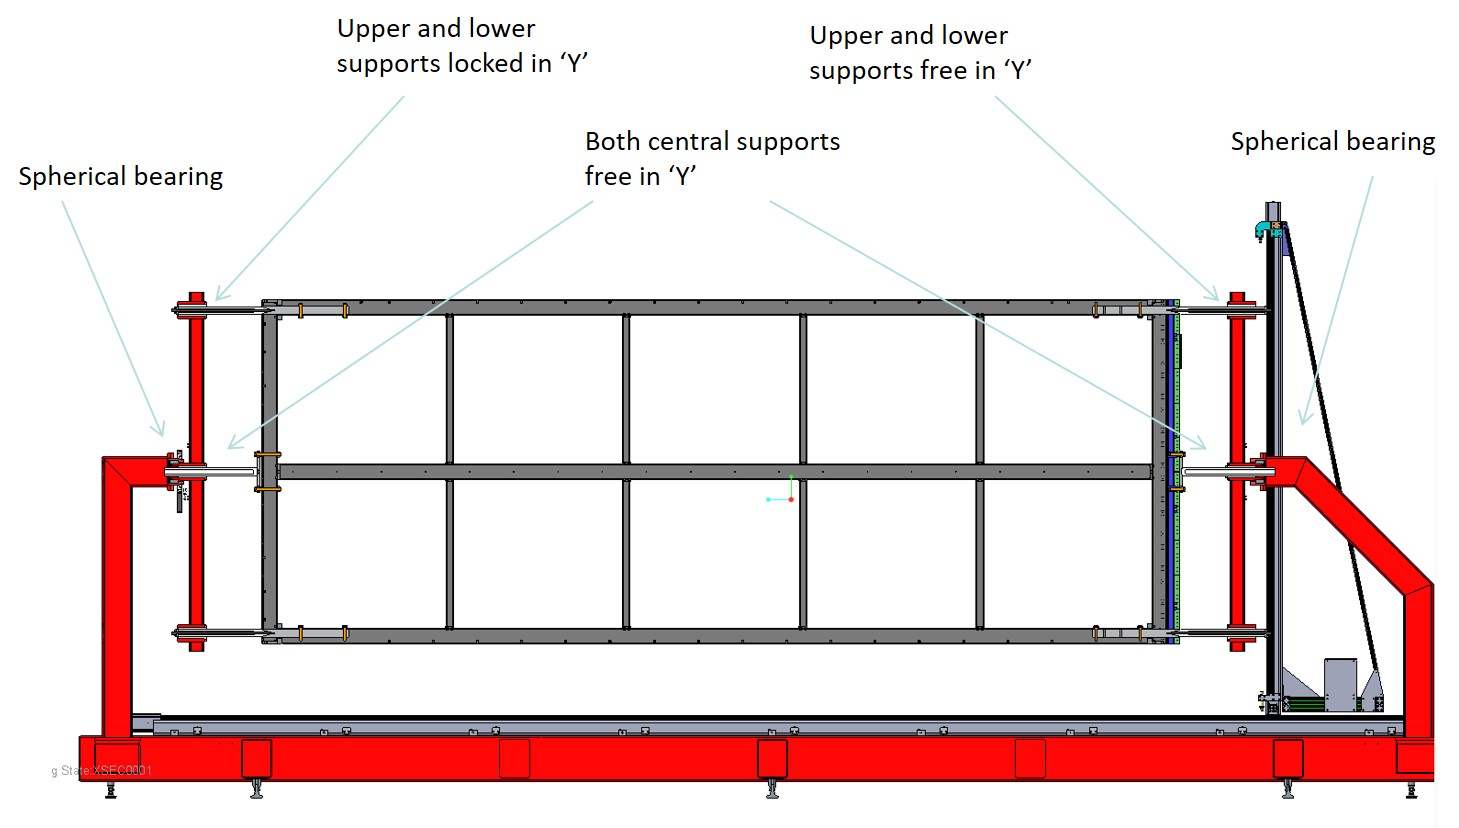
\includegraphics[width=0.95\textwidth]{sp-apa-winding-machine-design-development.jpg} 
\end{dunefigure}

\begin{dunefigure}[Photos of the \dword{apa} wire winding machine]{fig:winder-photos}
{Left: Partly wired \dword{pdsp} \dword{apa} on the winding machine at Daresbury Lab, UK. Right: Partly wired \dword{pdsp} \dword{apa} on the winding machine during wire tension measurements at University of Wisconsin, PSL.}
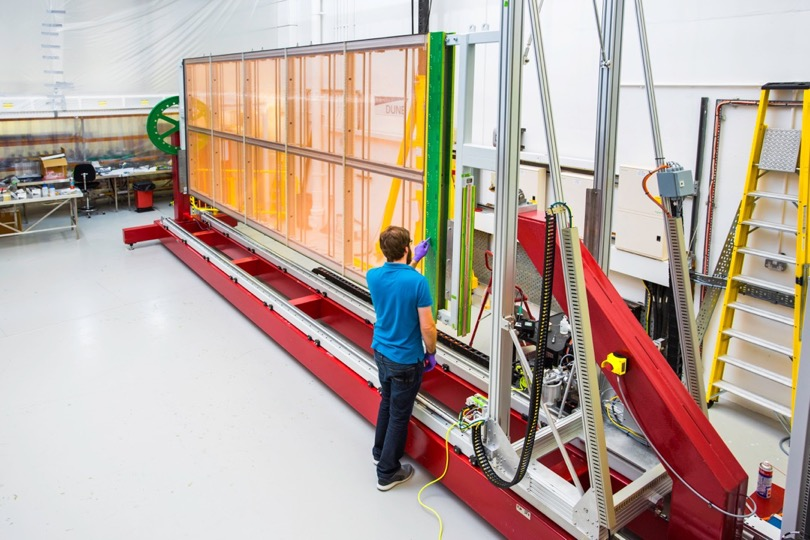
\includegraphics[height=0.3\textheight,trim=25mm 0mm 4mm 0mm,clip]{sp-apa-on-winder-daresbury.jpg}
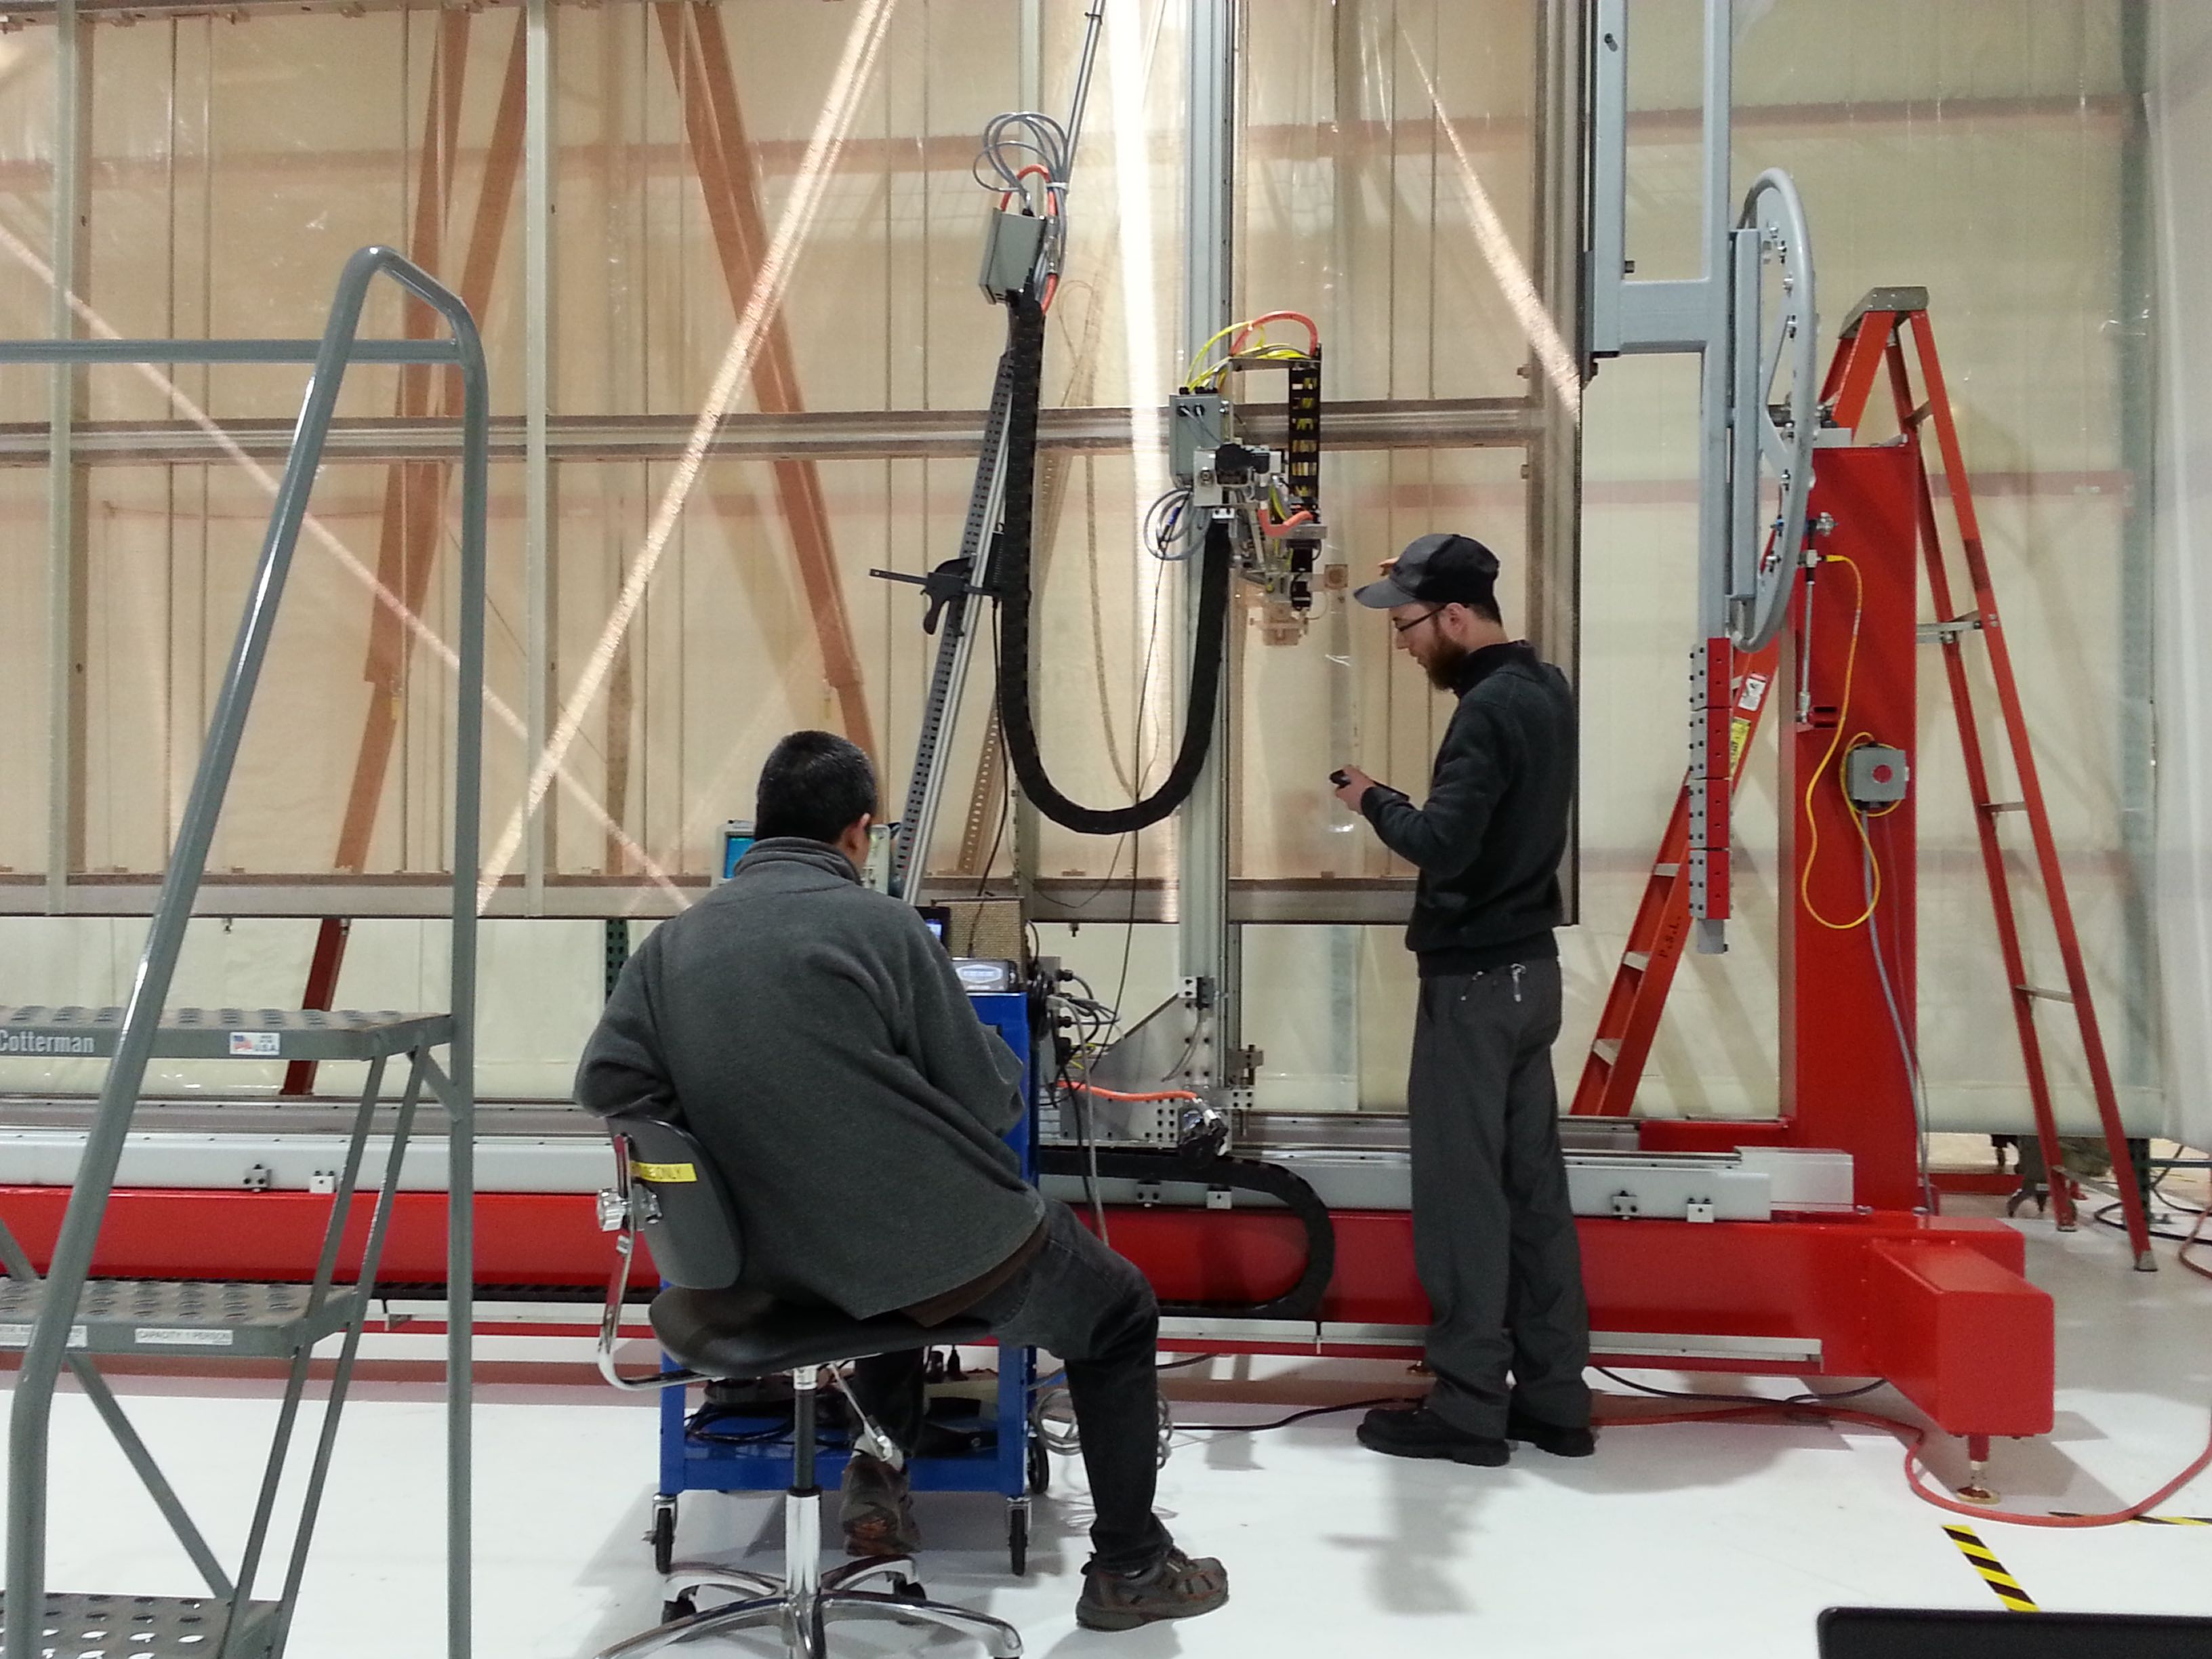
\includegraphics[height=0.3\textheight,trim=200mm 0mm 30mm 0mm,clip]{sp-apa-tension-testing-psl.jpg}
\end{dunefigure}

In the scheme used for \dword{pdsp}, during the winding process, an \dword{apa} moved on and off the winder machine several times for wiring, soldering, and testing, which is time consuming and increases risk.  Several design changes have been developed in 2018 to enable the \dword{apa} to remain on the winding machine throughout the wiring process. The design concept allows the winder head to pass from one side to the other nearly continuously. The interface frames at either end have been replaced by retractable linear guided shafts. These can be withdrawn to allow the winding head to pass around the frame over the full height of the frame. These shafts have conical ends and are in shafts fixed to the internal frame tube to provide guides to location. This design change does not alter the design of the frame itself, but it does allow for rotation in the winding machine. Thus, it is now possible to carry out board installation, gluing, and soldering in the winding machine. This eliminates any transfer of the APA to the process cart for the entire production operation, which is an inherently safer and faster production method because it cuts down on handling of the APA.  The upgraded design has been implemented on the winding machine at Daresbury, which is currently being used to build a new prototype, APA-07. All winding, board installation, gluing, soldering and testing operations are being carried out in the winding machine. APA-07 also incorporates the pre-built grounding mesh sub-frames, another new feature since the \dword{pdsp} design that saves significant time in production.  

\begin{dunefigure}[Photos of the upgraded \dword{apa} wire winding machine]{fig:winder-upgrade-photos}
{Left: Upgraded winding machine with new interface arm design being used to wire APA-07. Fitted mesh panels are also shown installed. Right: The V-layer soldering process at the head end of APA-07. Soldering can now be done with the \dword{apa} in the winding machine.}
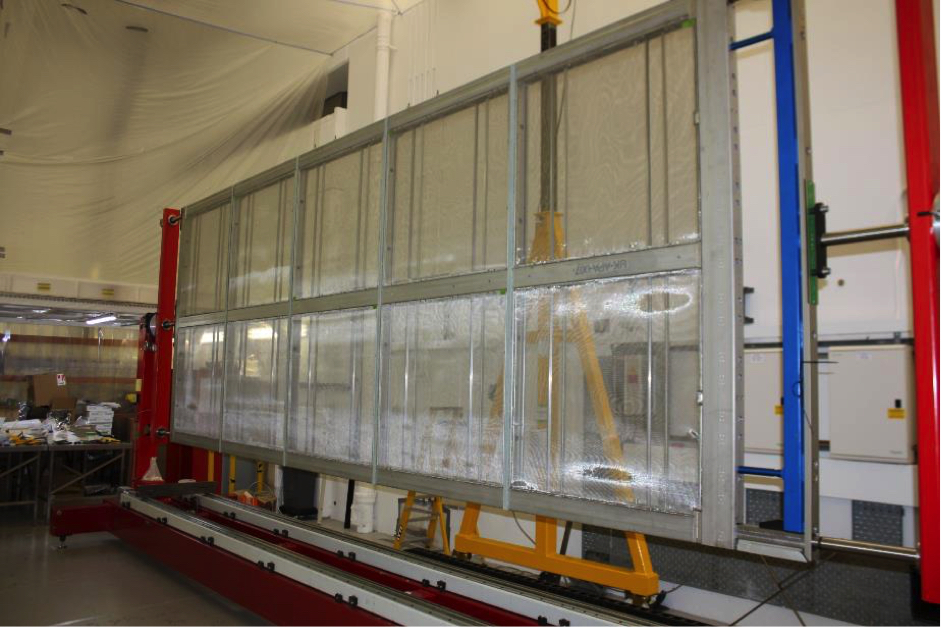
\includegraphics[height=0.24\textheight,trim=0mm 0mm 0mm 0mm,clip]{sp-apa-updated-winder.jpg} 
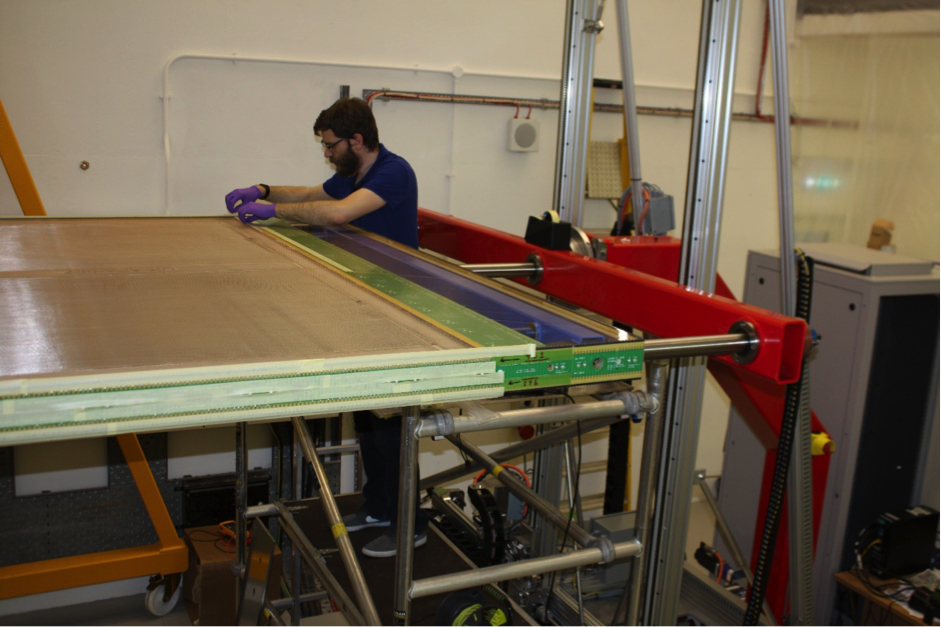
\includegraphics[height=0.24\textheight,trim=0mm 0mm 0mm 0mm,clip]{sp-apa-updated-winder-soldering.jpg}
\end{dunefigure}

Another important design effort since \dword{pdsp} construction has been to update the wiring head. The upgraded design offers real-time tension feedback and control, which will enable a big time savings in wiring and produce better tension uniformity across wires.  A prototype of the new head has been constructed and is undergoing extensive commissioning and qualification now and will be tested on a real \dword{apa} soon.     

One important element in the long-term use of the winders for making many \dword{apa}s for DUNE will be maintenance.  The approach to winder maintenance during \dword{pdsp} construction was not well considered. As a result, winding machine problems traceable to lack of routine maintenance occurred from time to time, shutting the production line down until repair or maintenance was performed. We will formulate a routine and preventive maintenance plan that minimizes winder downtime during \dword{apa} production.

Another key element in the flow of activities during production are large process carts, with an example shown in Figure~\ref{fig:apa-process-cart}. The process carts can be used to hold \dword{apa}s during wiring preparations and for quality control checks after wiring, and to safely move \dword{apa}s around within the assembly facility. 
%and also move them to a shipping/packing location area for loading into specialized crate containers. 
%One process cart with regular casters remains in the assembly area; it is kept at a particular height that coordinates with other construction tooling equipment like jack stands and platform ladders. 
Process carts are fitted with specialized 360$^\circ$ rotating casters that allow the cart, loaded with a fully assembled \dword{apa}, to maneuver corners while moving the large frames between preparation, assembly, and packing/shipping areas.

\begin{dunefigure}[Photo of an \dword{apa} on a process cart during construction]{fig:apa-process-cart}{A \dword{pdsp} \dword{apa} being moved around the PSL production facility on a process cart. 
%(Right) \dword{apa} frame with the grounding mesh already installed is shown sitting on a process cart.  Two technicians are using a custom jig to place the wire combs above a horizontal cross beam on the \dword{apa}.
}
%\setlength{\fboxsep}{0pt}
%\setlength{\fboxrule}{0.5pt}
%\fbox{\includegraphics[height=0.24\textheight,trim=50mm 0mm 70mm 0mm,clip]{apa-process-cart.jpg}}
%\fbox{\includegraphics[height=0.24\textheight,trim=15mm 0mm 35mm 0mm,clip]{apa-comb-base-jig.png}}
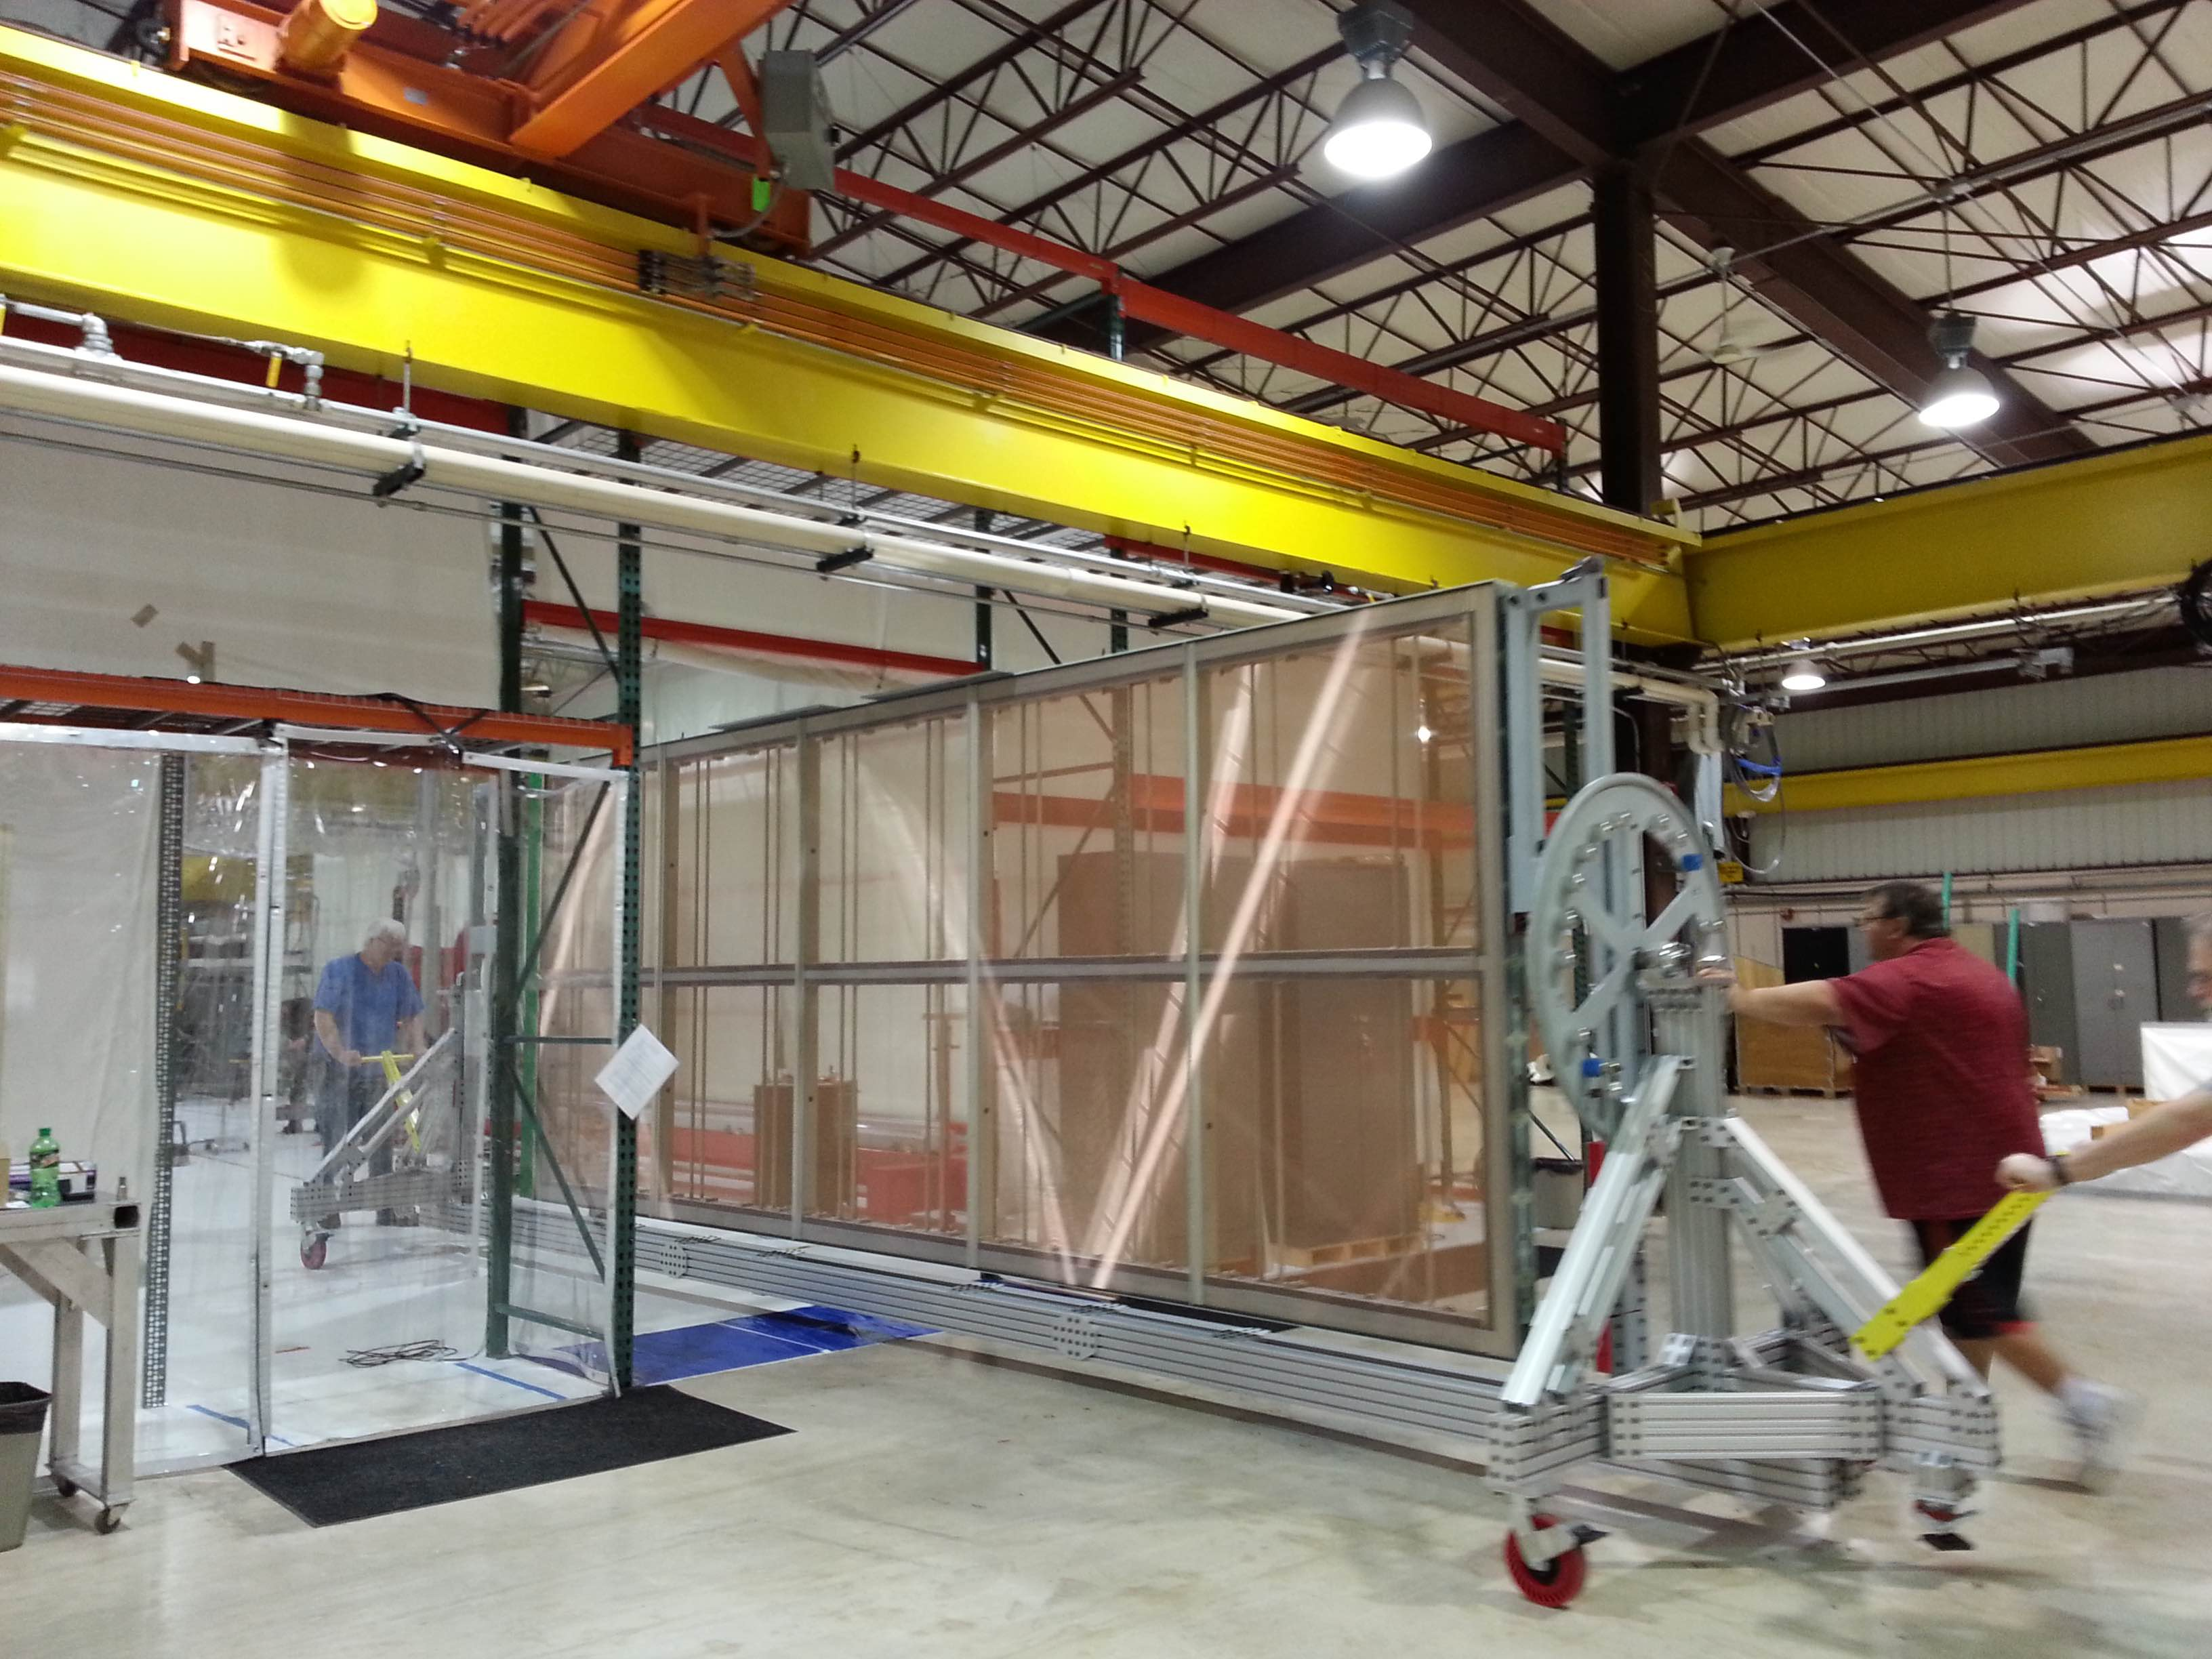
\includegraphics[height=0.3\textheight,trim=50mm 10mm 70mm 250mm,clip]{sp-apa-process-cart.jpg}
%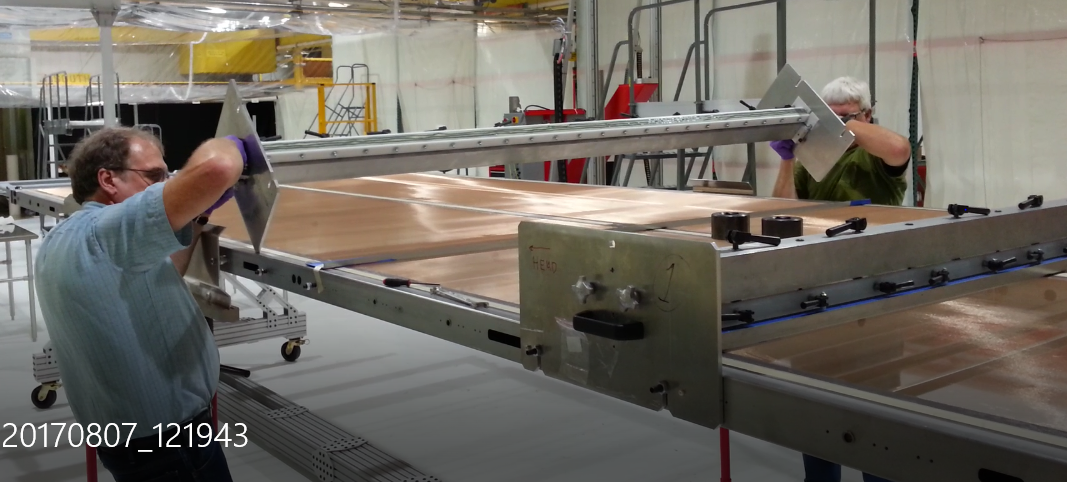
\includegraphics[height=0.23\textheight,trim=15mm 0mm 35mm 0mm,clip]{sp-apa-comb-base-jig.png}
\end{dunefigure}

%Before wiring can begin, the grounding mesh panels must be installed on the bare frame. 
%
%In the \dword{pdsp} design, a large jig holds the mesh in place for gluing. Once the jig is sufficiently leveled to the frame, a mesh sheet is laid into place and hold down bars are iteratively moved and repositioned until the mesh is flat and tight.  The outside edge of the mesh panel is then epoxied, and the jig and hold down bars remain in place for a 12 hour epoxy cure cycle.  This process is then repeated for the next three shifts until all four panels of mesh have been attached to the bare \dword{apa} frame.  As described below, we are considering changes to this lengthy procedure for DUNE \dwords{apa}.  

%Another custom construction jig is needed to install the wire combs that hold the wires at intermediate points above the four cross beams of the \dword{apa}.  Currently, two jigs can be loaded and installed at a time, and each installation requires a six-hour epoxy cure cycle. %the two jigs are removed from the initial locations and placed in another two locations, on the same side of the \dword{apa}.  Thus four comb bases are installed within one operation shift and the \dword{apa} is left in this horizontal position to cure overnight.  The next day, the \dword{apa} is flipped to the reverse side and the process is repeated for the other side. Figure~\ref{fig:apa-process-cart} shows the comb installation jig in use.  

%\subsubsection{Planned Improvements to Production Process}


Based on the \dword{pdsp} experience, we have identified a few other areas for potential improvement to the construction process that could make \dwords{apa} fabrication more efficient and reliable.   The first is the wire tension measurement technique. The current technique uses a laser photodiode tool mounted on the winder to measure tension one wire at a time. This takes many hours for each wire plane. A task force within the Consortium was recently initiated to study the problem and consider possible new approaches to measuring tension.  In particular, methods to electronically measure groups of \num{20} or more wires at one time have recently been explored, so the task force is studying the feasibility of applying this during \dword{apa} construction. With a less labor intensive and faster method, it also becomes possible to measure more of the wire tensions later in the lifetime, for example at the \dword{itf}.  


%\begin{itemize}

%\item Wiring head design: Efforts to improve winder head performance are already underway. We envision improved tension control, continuous tension feedback, improved clutch, and improvement to the compensator mechanism, all leading to better, more consistent, and more reliable winder performance.  The current winding head uses a magnetic clutch mechanism that is manually adjusted to increase or decrease the tension of the wire as it is wound around the \dword{apa}. The clutch regularly needs adjustment because the diameter of the wire on the spool declines during the winding process. In addition, if the mechanism is run from a cold start, the tension changes after $\sim$10 minutes of running. Experience winding the \dword{pdsp} \dwords{apa} has shown that maintaining the target tension within tolerances (5$\pm$\SI{1}{N} for \dword{pdsp}) is difficult.

%A solution to this issue is to design a winder head with active tension control by replacing the magnetic clutch with a servo motor and introducing a potentiometer on a dancer arm for the feedback loop (see Figure~\ref{fig:winding-head}). This only works if no signal losses occur when transferring the winding head to the compensator latching mechanism and back. The system can be driven in torque mode and should compensate for any wire spool changes. It must be able to operate from a cold start. This development is well underway, and the changes are being tested.

%\begin{dunefigure}[Exploded view of the winding machine head]{fig:winding-head}
%{Exploded view of winder head with active tension control.}
%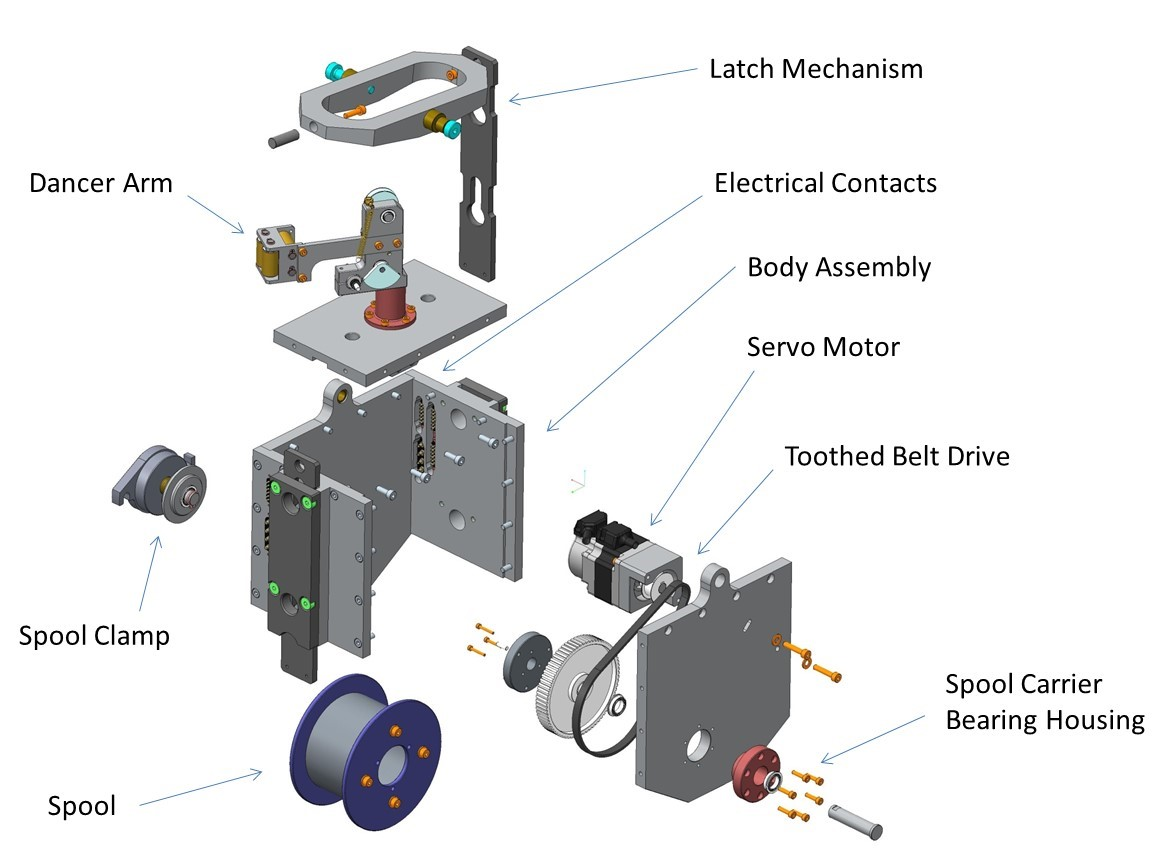
\includegraphics[width=0.7\textwidth]{sp-apa-winder-head-with-active-tension-controls.jpg}
%\end{dunefigure}

%\item Winder interface arm design: The current winder interface only allows one-half of a wire plane to be wired at a time. The \dword{apa} frame must be moved to the process cart where the interface arms are flipped 180$^\circ$ to wind the second half of the wire plane.  A new design concept, illustrated in Figure~\ref{fig:winding-dev}, allows the winder head to pass from one side to the other nearly continuously without removing the frame from the winding machine.  The interface frames are replaced at either end by retractable linear guided shafts. These can be withdrawn to allow the winding head to pass around the frame over the full height of the frame. These shafts have conical ends and are in shafts fixed to the internal frame tube to provide guides to location. This design change does not alter the design of the frame itself, but it does allow for rotation in the winding machine. Thus, it should also be possible to carry out board installation, gluing, and soldering in the winding machine. This eliminates any transfer of the \dword{apa} to the process cart for the entire production operation, which is an inherently safer and faster production method because it cuts down on handling the \dword{apa}.

%\item Modular mesh panels: The current approach to mesh installation is slow and cumbersome. We will improve this part of construction by moving toward a modular window screen design that improves the reliability of the installed mesh (more uniform tension across the mesh) and allows much easier installation on the \dword{apa} frame.

%\fixme{Can you please check the following paragraph? I was interrupted while working on it, and I'm afraid it's not accurate any more.}

%\item Epoxy process improvements: Applying epoxy during the construction process requires many steps. These steps require careful work and many hours between winding each successive wire plane as the epoxy cures. We already have concepts for improving epoxy application jigs from \dword{pdsp}, and we will investigate whether epoxy pre-forms or accelerated heat curing can improve time or reliability.

%\item Automated soldering: Every solder joint on the six \dword{pdsp} \dwords{apa} was done by hand. We will investigate automated soldering techniques to improve the process and reduce the amount of manual effort required. 

%\item Wire tension measurement techniques: Verifying wire tension during construction is an important, but time consuming, process. The current technique uses a laser photodiode tool mounted on the winder to measure tension one wire at a time. This takes many hours for each wire plane. Collaborators at the University of Manchester are developing techniques to electronically measure groups of \num{20} or more wires at one time. This technique provides much faster tension measurements and shorter turnaround between wire planes. 

%\item Winder maintenance plan: The approach to winder maintenance during \dword{pdsp} construction was not well considered. As a result, winding machine problems traceable to lack of routine maintenance occurred from time to time, shutting the production line down until repair or maintenance was performed. We will formulate a routine and preventive maintenance plan that minimizes winder downtime during \dword{apa} production.
%\end{itemize}


%%%%%%%%%%%%%%%%%%%%%%%%%%%%%%%%%%%%%%%%%%%%%%%%%%%%%%%%%%%%%%%%%%%%%%%%%%%
\subsection{\dword{apa} Construction Facilities}
\label{sec:fdsp-apa-prod-facility}
%%%%%%%%%%%%%%%%%%%%%%%%%%%%%%%%%%%%%%%%%%%%%%%%%%%%%%%%%%%%%%%%%%%%%%%%%%%

Construction of \dword{spmod} \dwords{apa} will take place in both the USA and the UK.  Multiple \dword{apa} production lines spread over several facilities will provide some margin on the production schedule and provide back up in the event that technical problems occur at any particular site. 
%\fixme{specified future partner sites}

The space requirements for each production line are driven by the size of the \dword{apa} frames and the winding robot used to build them. The approximate dimensions of a class \num{100000} clean space needed to house winder operations and associated tooling is \SI{175}{m$^2$}. The estimated requirement for inventory, work in progress, and completed \dwords{apa} is about \SI{600}{m$^2$}. Each facility  also needs temporary access to shipping and crating space of about \SI{200}{m$^2$}. Possible floor layouts at each institution are being developed. Adequate space is available at each site, and the institutions have offered commitments for space for DUNE. 

At Daresbury Laboratory in the UK the existing single production line used for \dword{pdsp} construction will be expanded to four.  The ``Inner Hall'' on the Daresbury site has been identified as an area that is large enough to be used for DUNE \dword{apa} construction. It has good access and crane coverage throughout. Daresbury Laboratory management have agreed that the area is available, but a safe working environment will require some investment. Preparation for construction is underway, clearing the current area of existing facilities, obsolete cranes, and ancillary equipment. The renovation of a plant room is also planned, so it can be used for storage and as a shipping area. This work is ongoing. The production factory is being designed to hold four winding machines and associated process equipment and tooling.  

\begin{dunefigure}[Layouts of \dword{apa} factories]{fig:factories}
{Developing concepts for factory layouts at Daresbury Lab (top left), University of Chicago (top right), and Yale University (bottom left), and the existing APA production area at PSL-Wisconsin (bottom right).}
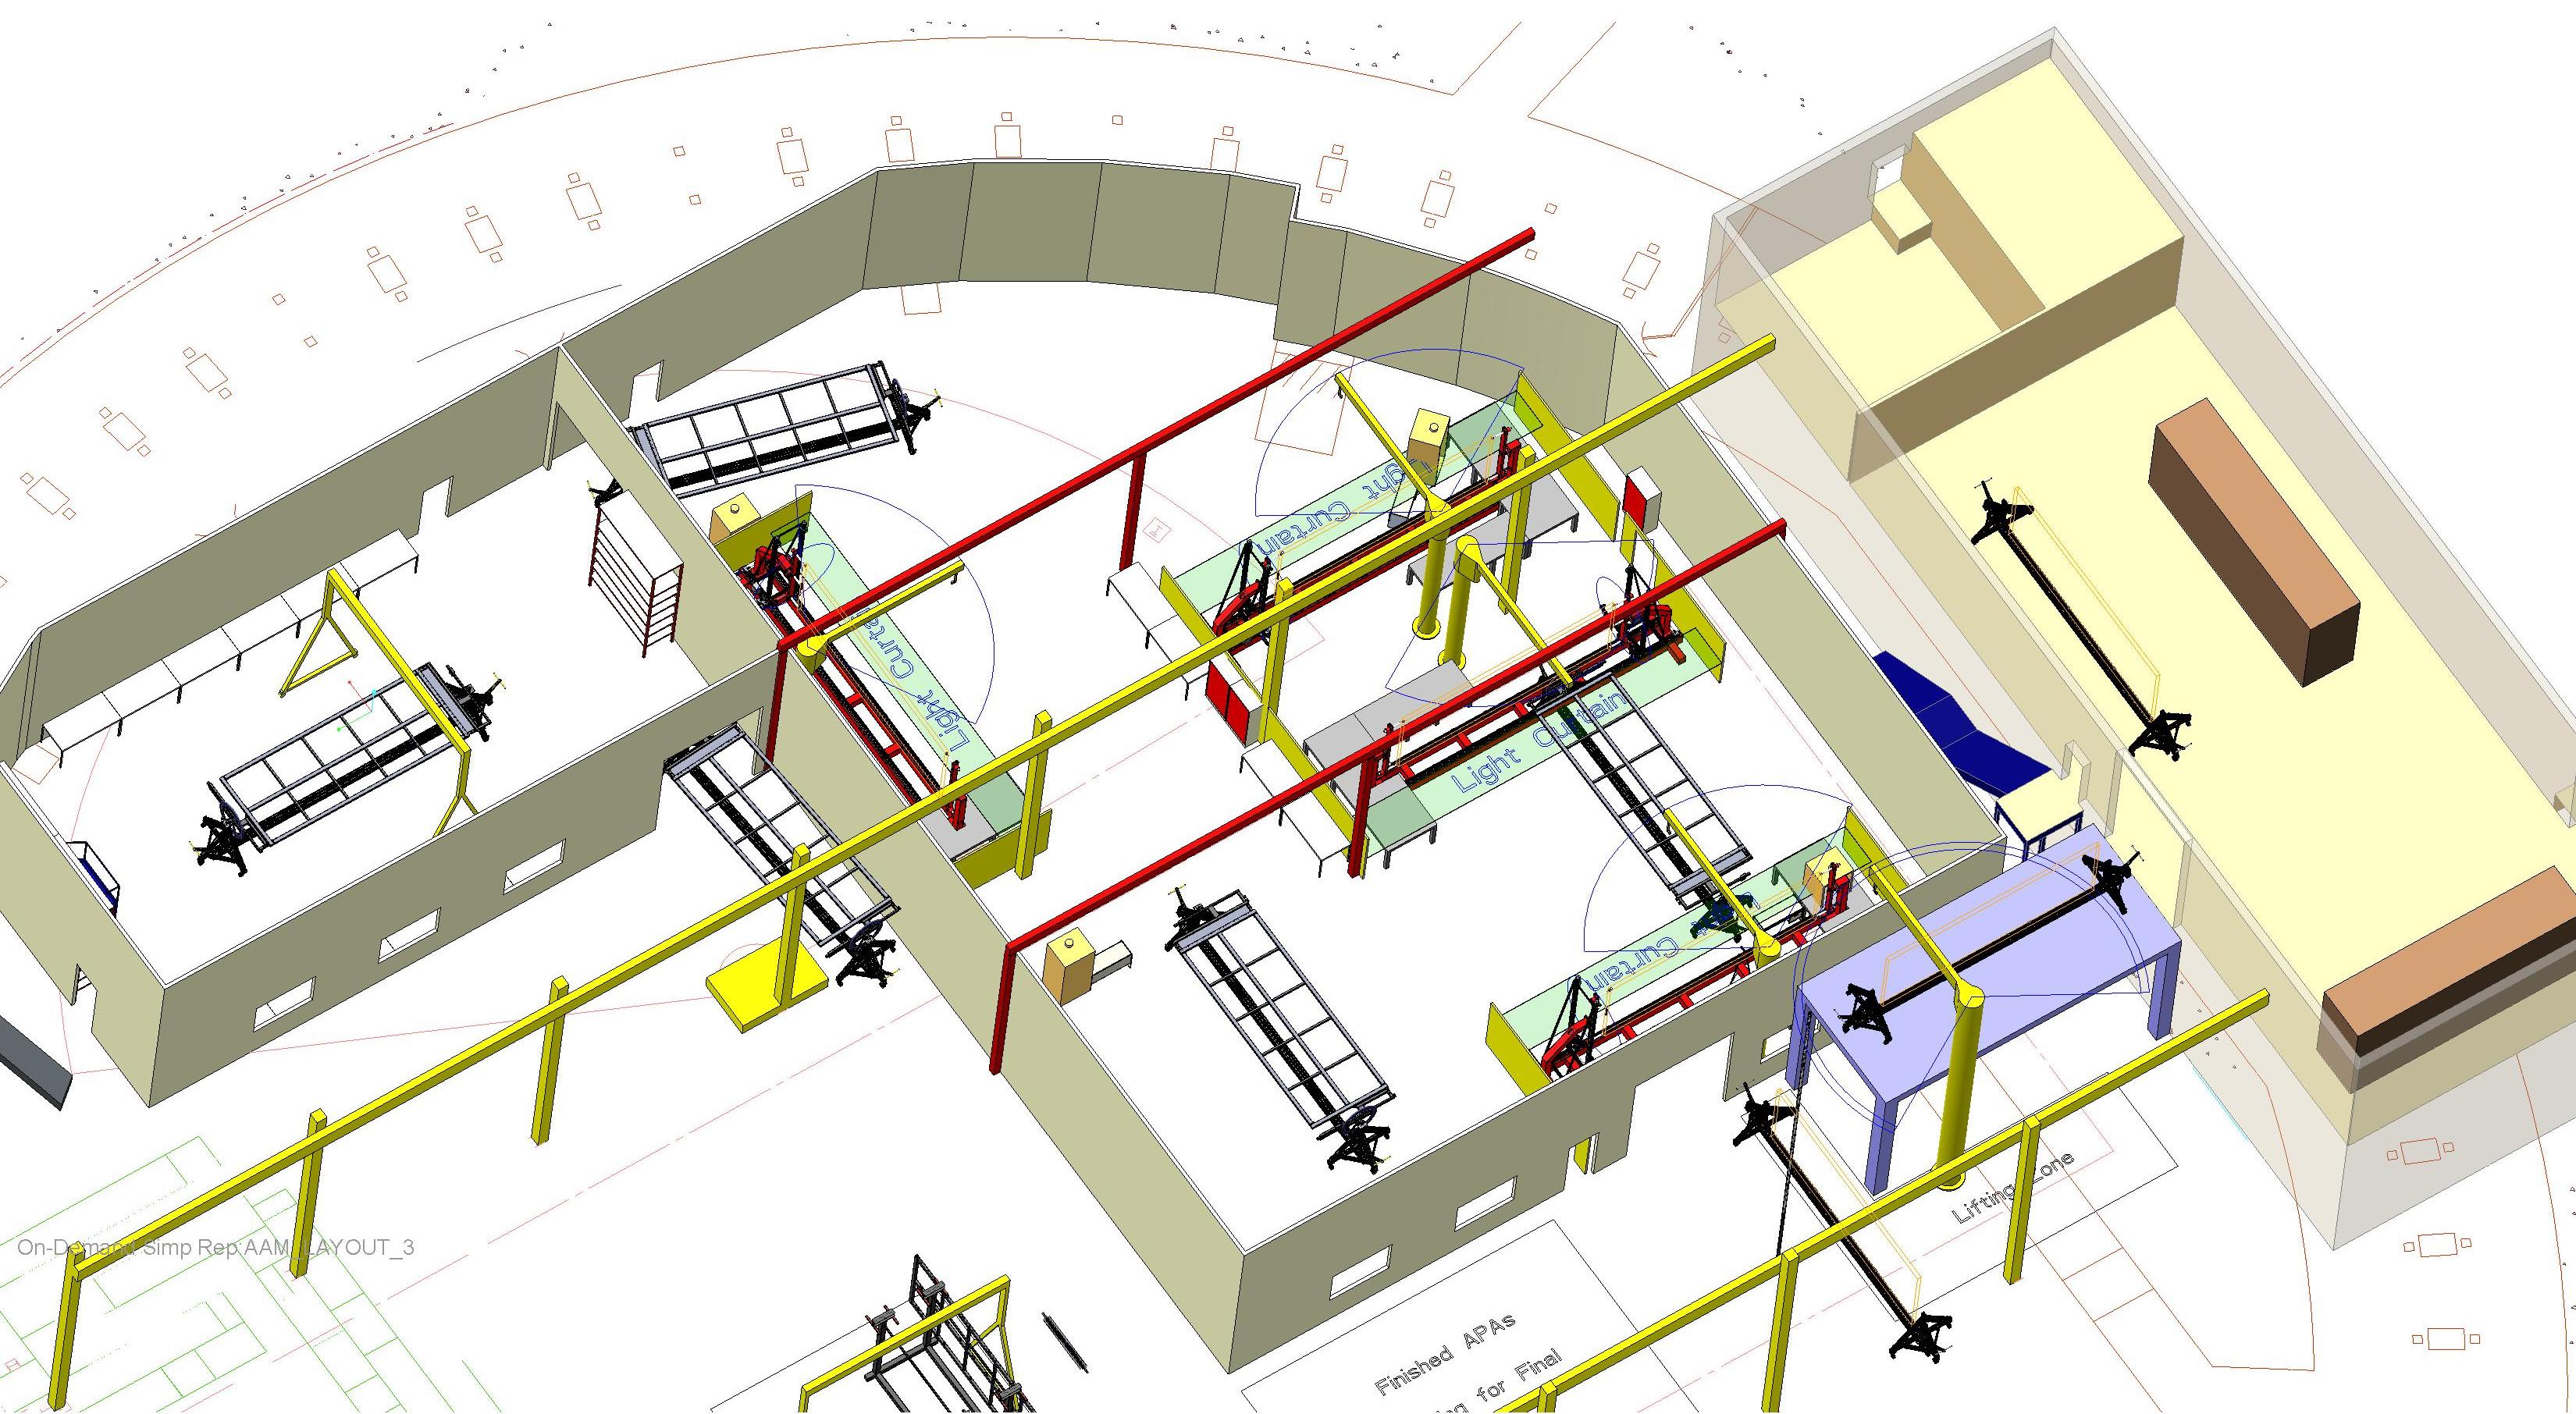
\includegraphics[height=0.23\textheight]{sp-apa-factory-daresbury.jpg} 
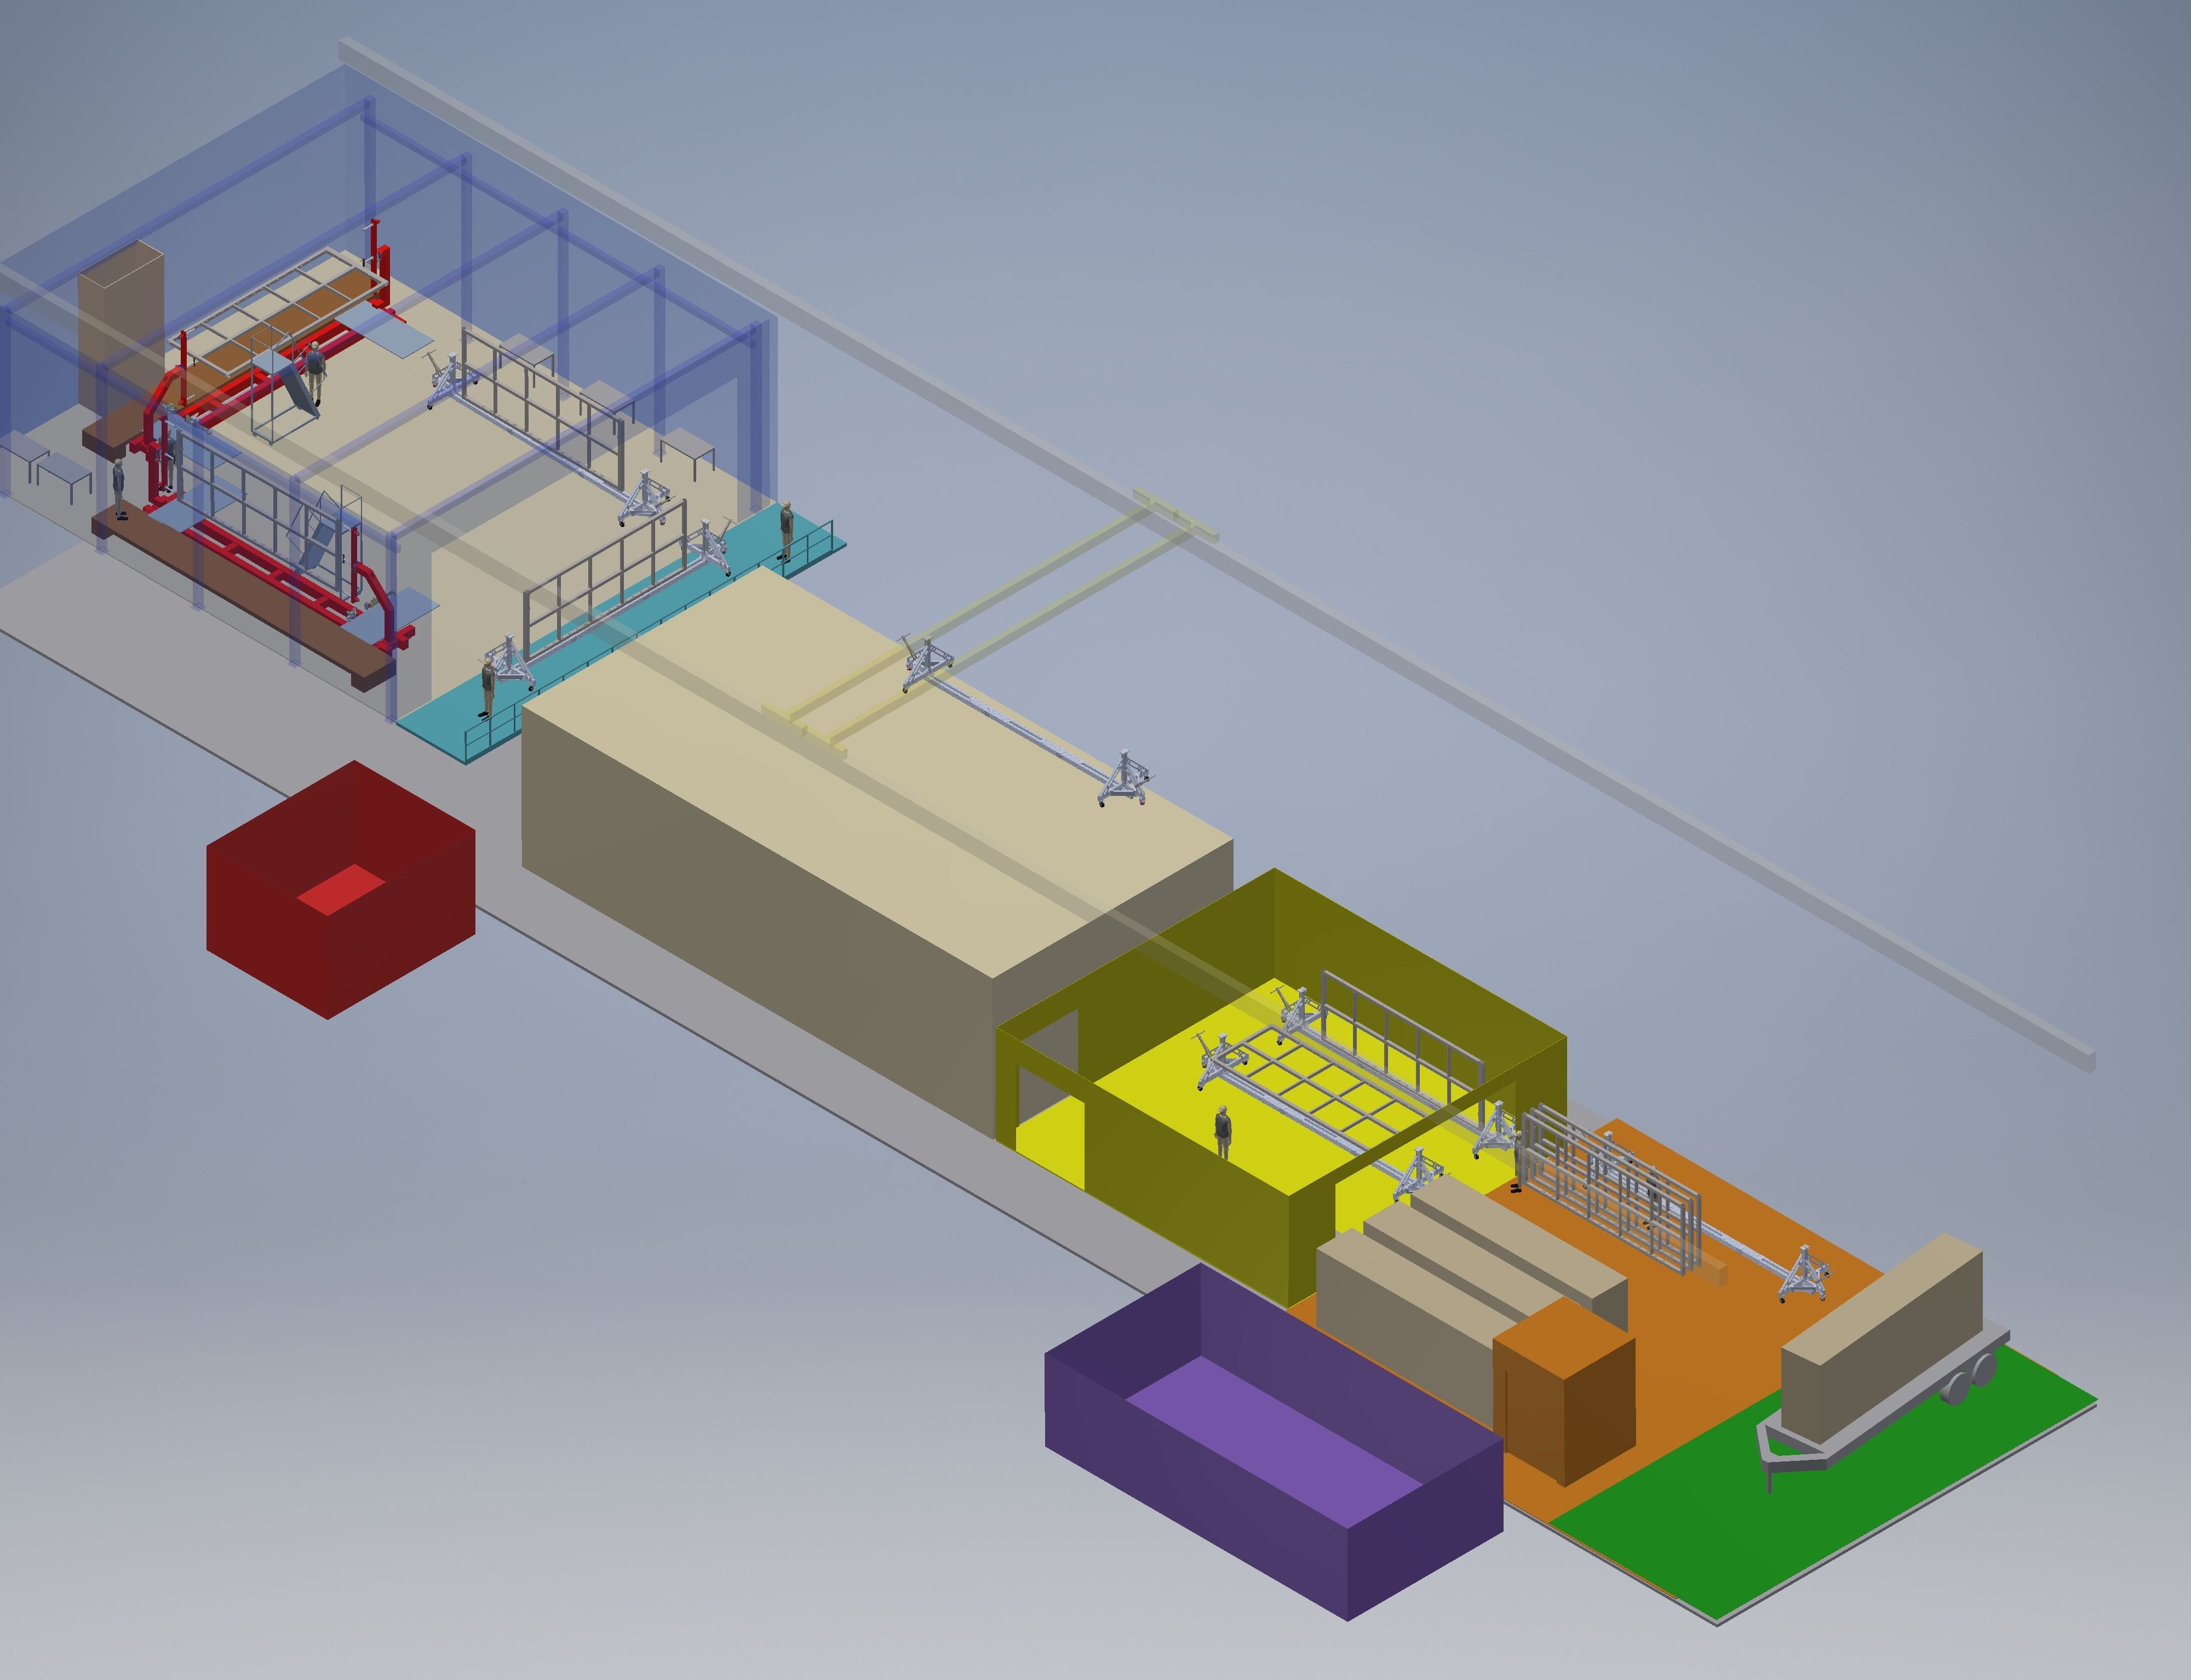
\includegraphics[height=0.23\textheight]{sp-apa-factory-chicago.jpg} \\
\vspace{1mm}
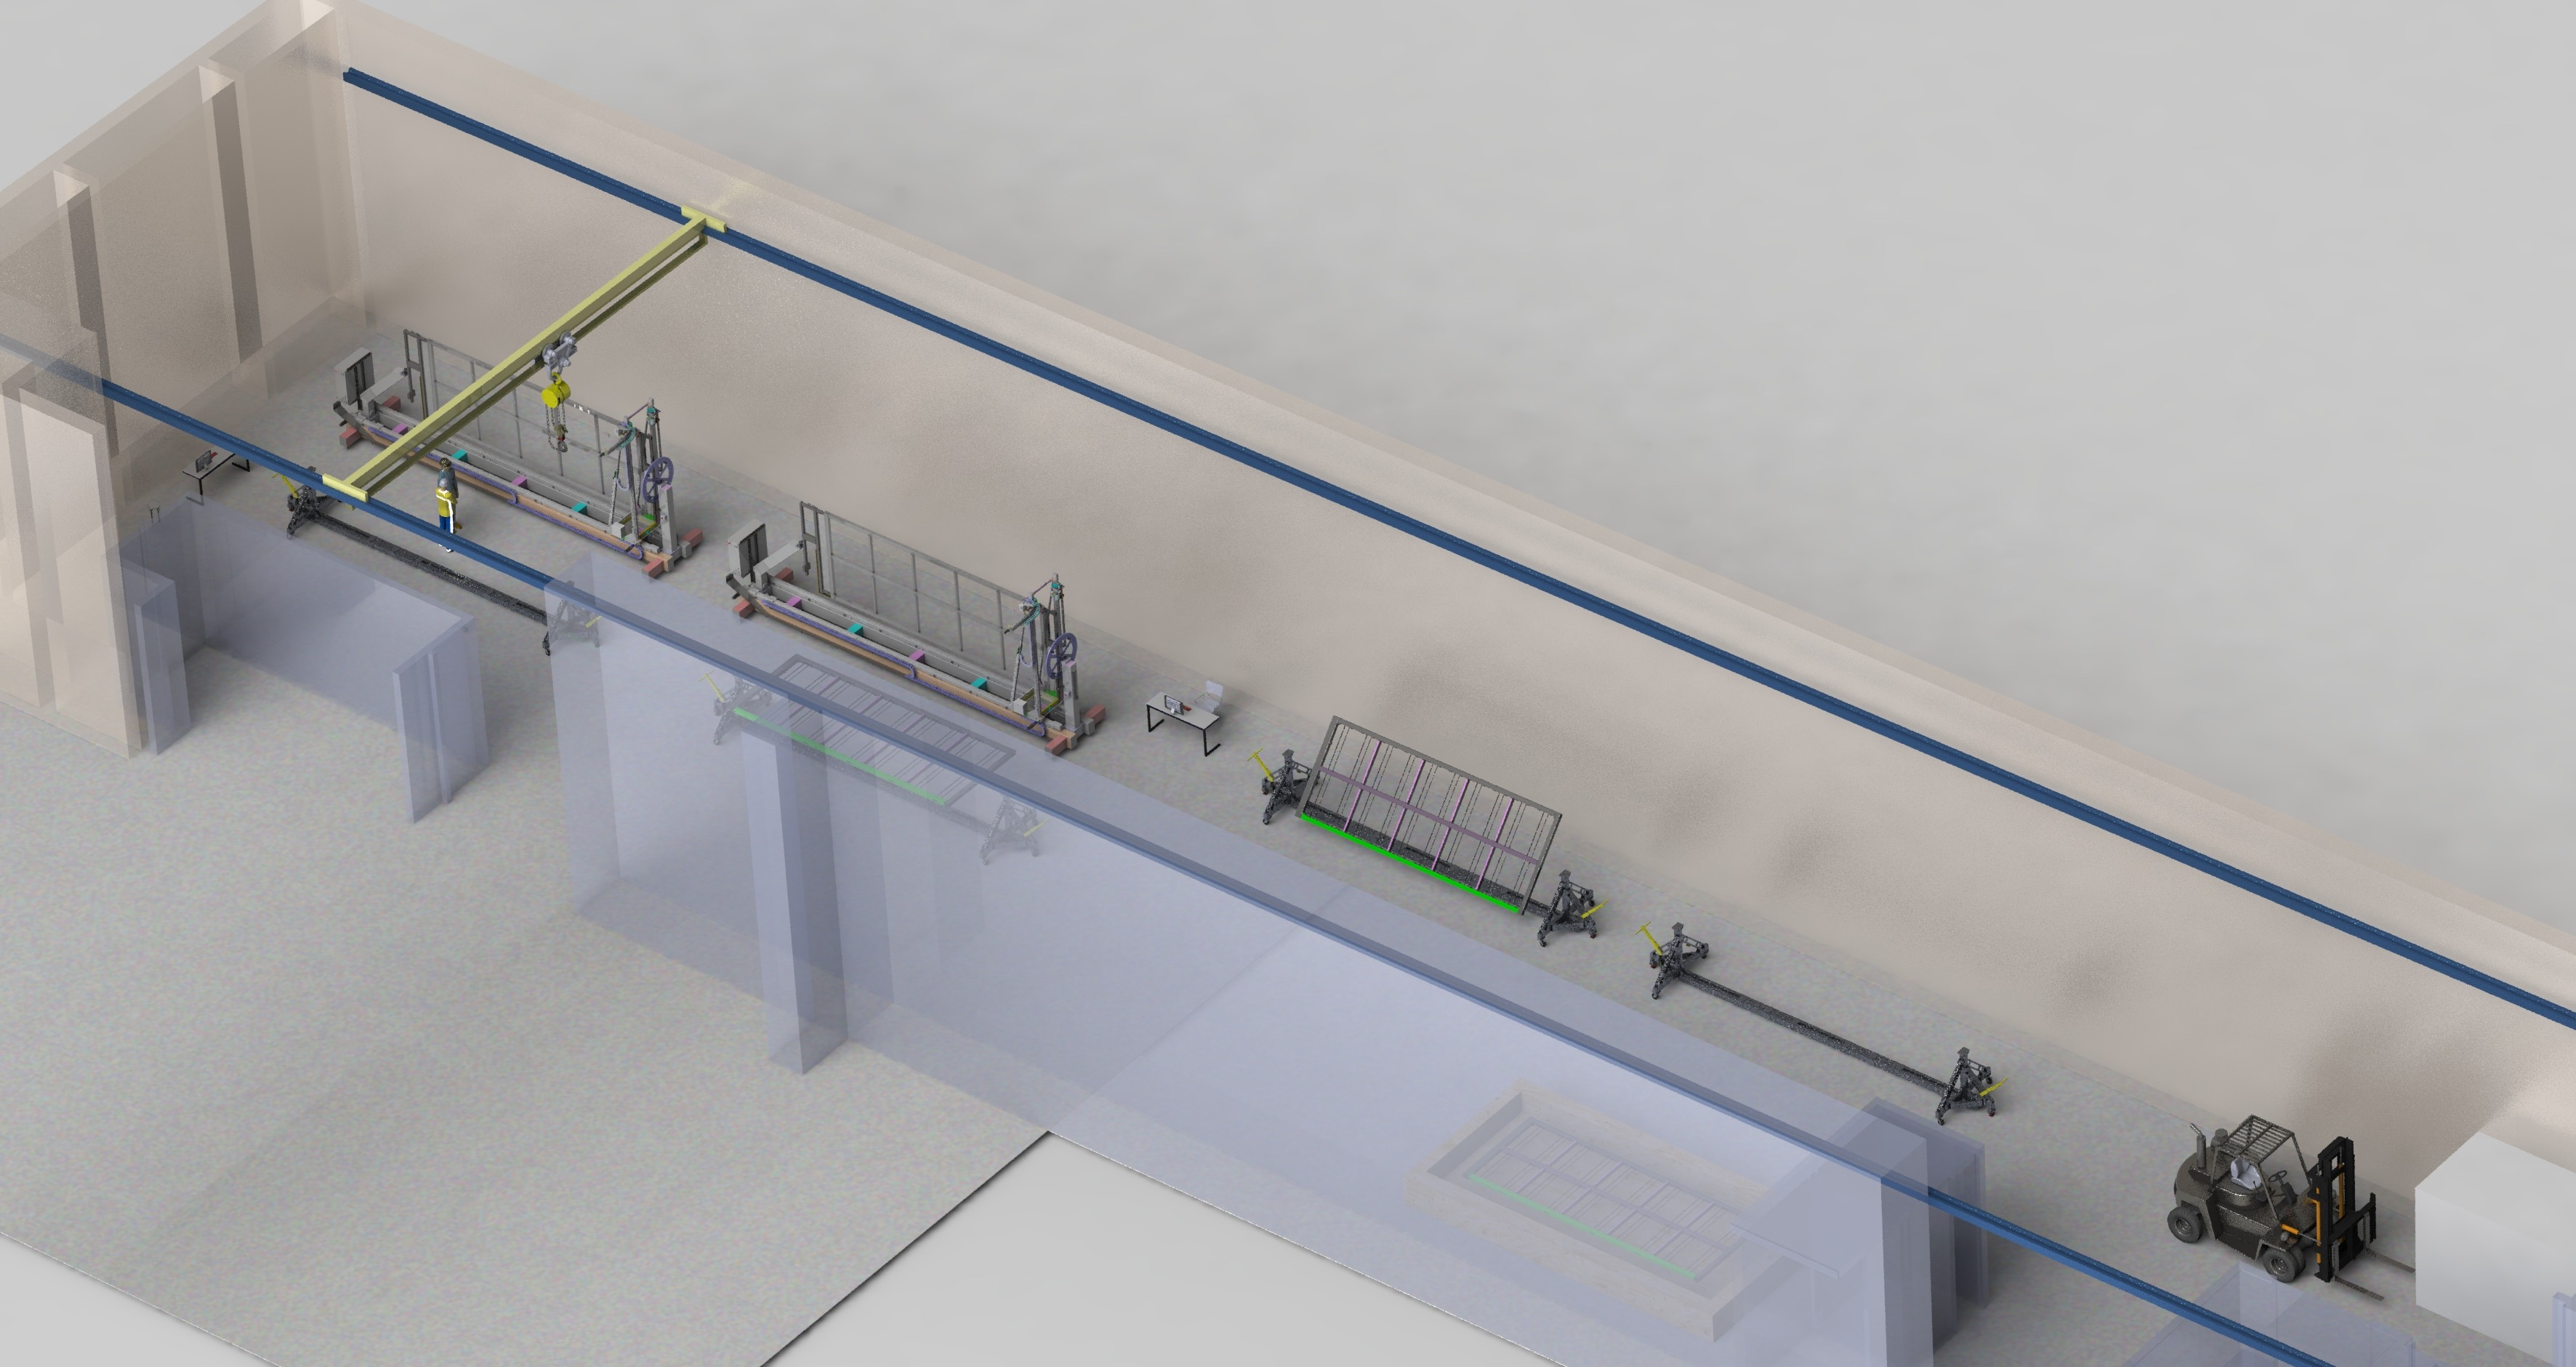
\includegraphics[height=0.225\textheight]{sp-apa-factory-yale.jpg}
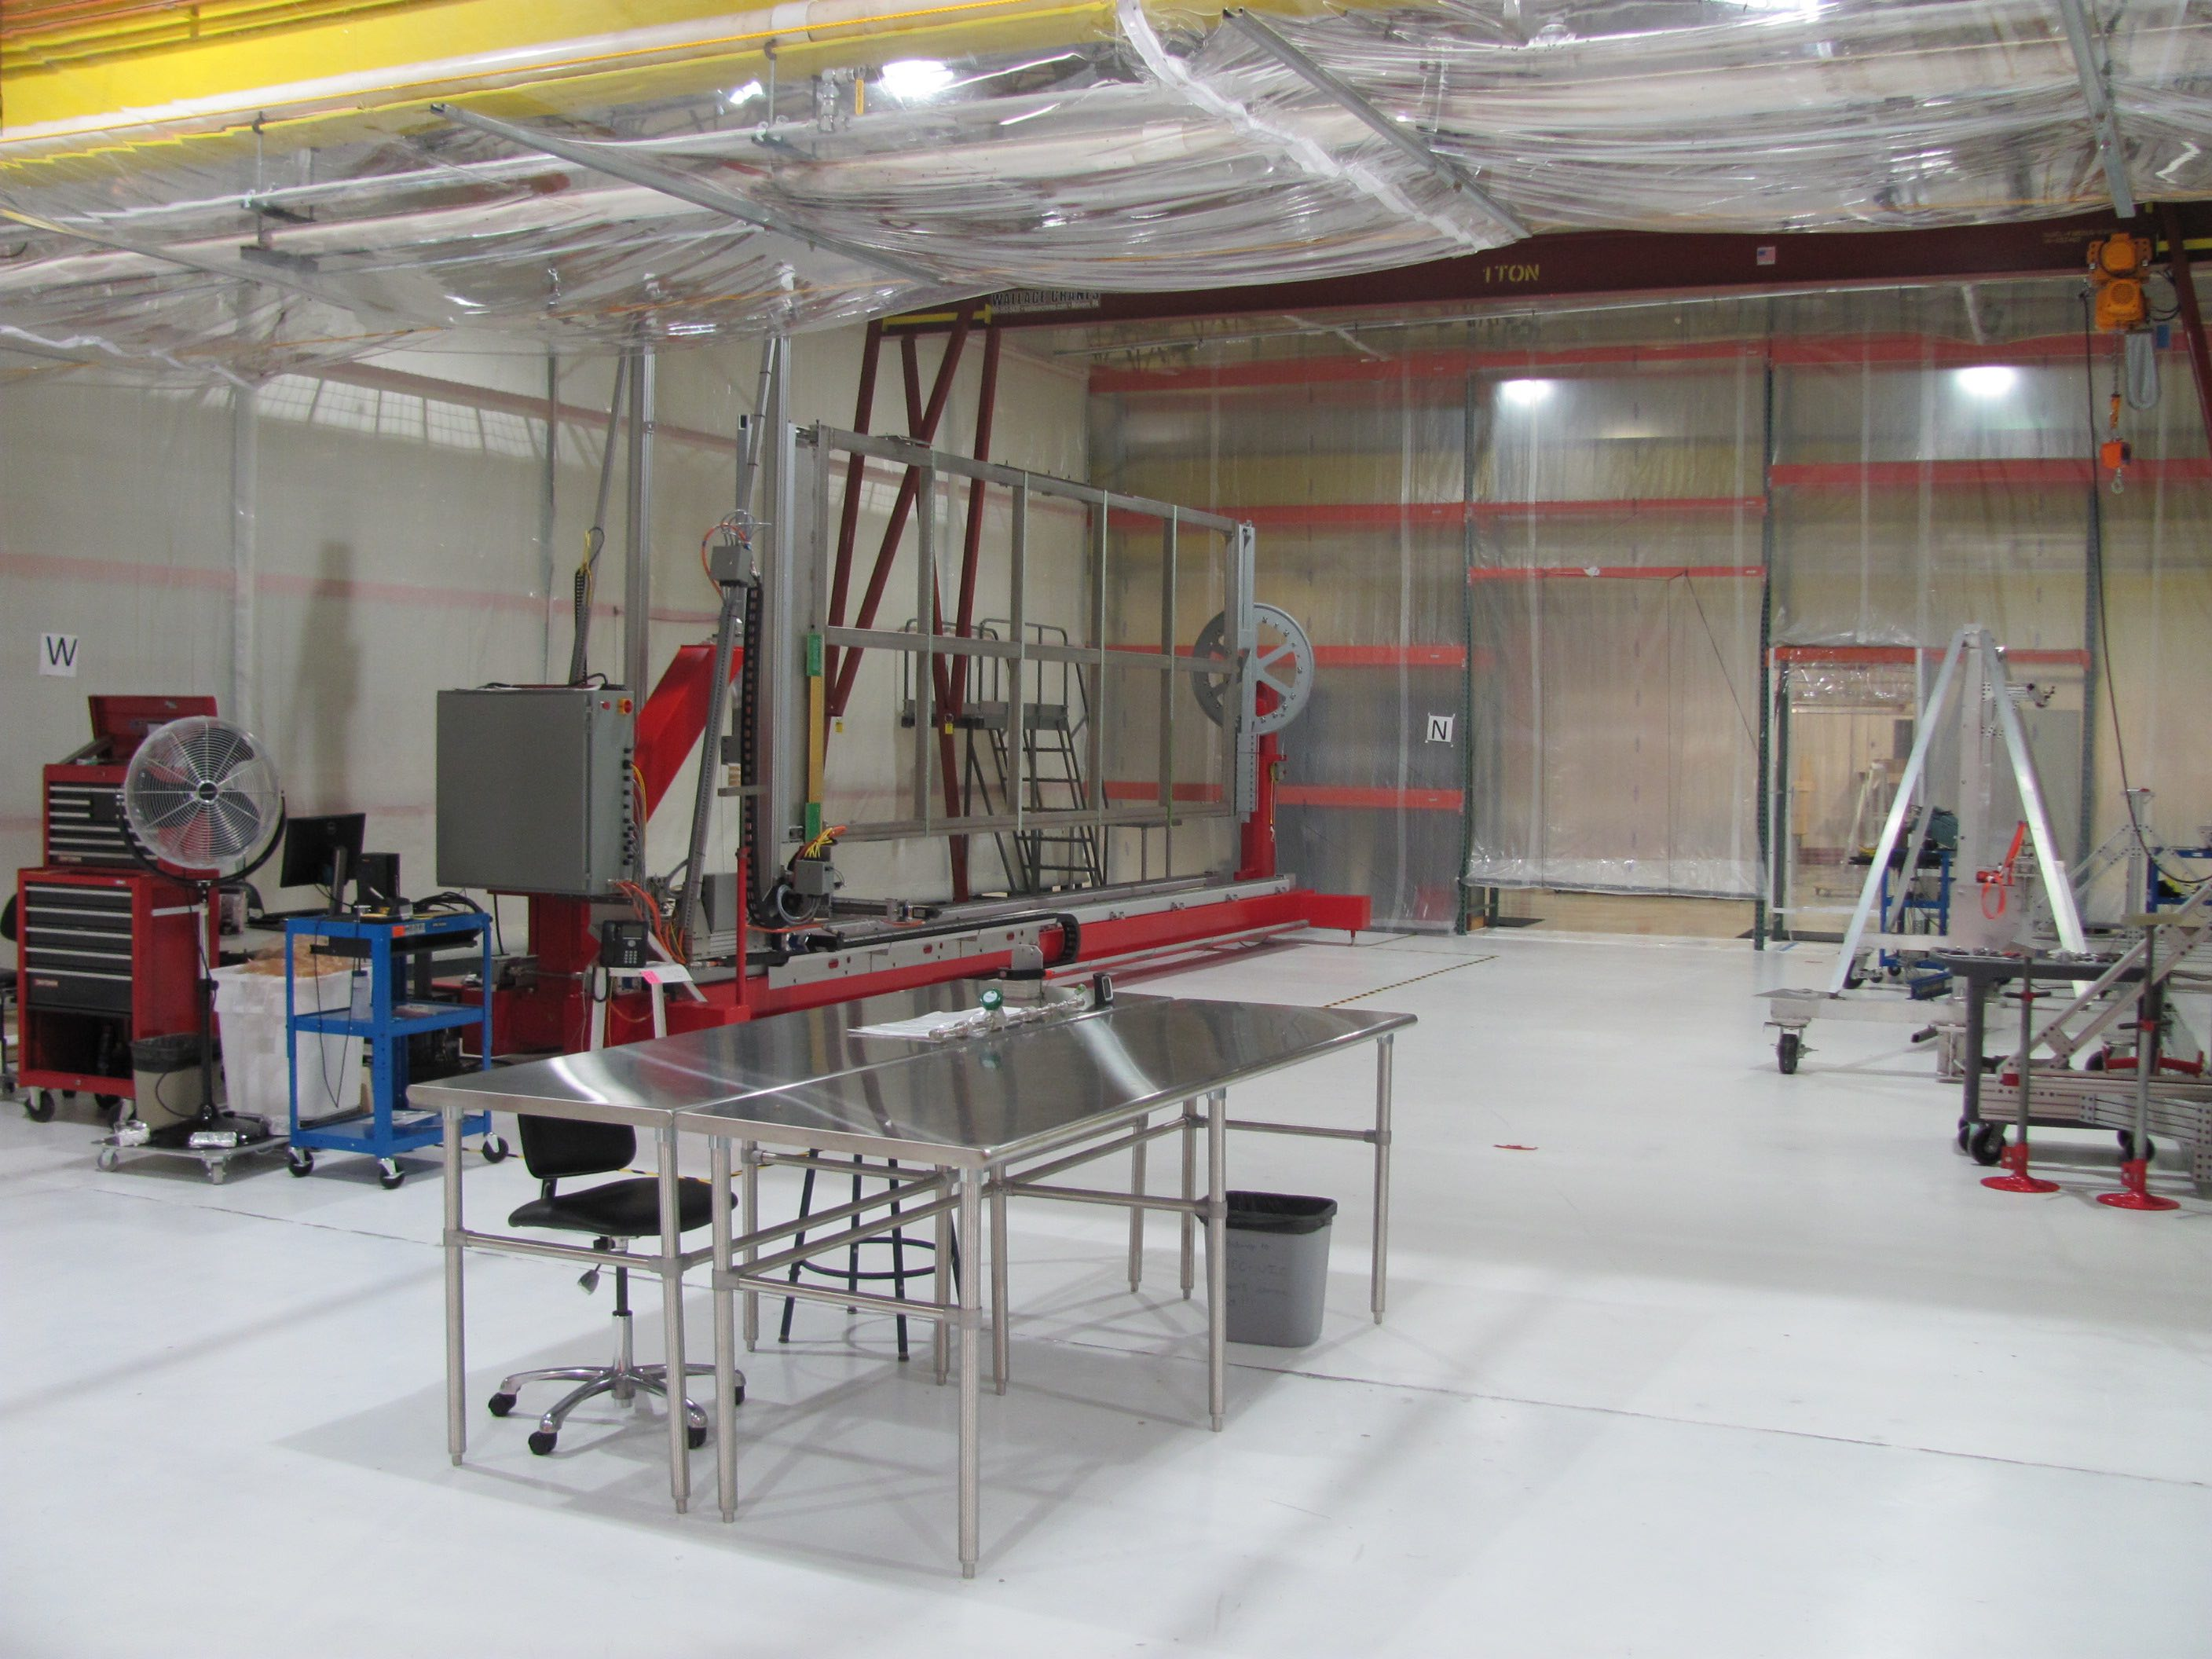
\includegraphics[height=0.225\textheight]{sp-apa-factory-psl.jpg} 
\end{dunefigure}

In the US, there will be five total production lines at three facilities at the University of Chicago (2), Yale University (2), and the already existing production line at the University of Wisconsin (1). The University of Wisconsin has space available in the Physical Sciences Laboratory (PSL), Rowe Technology Center, where the construction for \dword{pdsp} has been carried out, with up to \SI{20000}{ft^2} (\SI{1850}{m^2}) total space available for continued DUNE activities. 

The APA factory at the University of Chicago will be housed in the Accelerator building on campus in Hyde Park.  The building has hosted assembly of large apparatus for numerous experiments over the course of its history and features an extensive high bay with an overhead crane, an indoor truck bay, clean laboratory spaces, a professional machine shop, and proximity to faculty and staff offices.  Winding will be done inside a clean room installed on the first floor-level mezzanine, where there is \SI{234}{m^2} of floor space, above the machine shop.  A \SI{2}{ton} capacity bridge crane will be installed inside this clean room to move \dword{apa}s to and from the two winders and process carts that will be located here.  \dword{apa}s will enter and exit the mezzanine by way of a loading deck external to the clean room.  Preparation of \dword{apa} frames, including mesh installation, will be done inside a second clean room on the basement level floor of the high bay.  Ample space, roughly \SI{170}{m^2}, between this clean room and the truck bay allows for simultaneous receiving of bare frames or other larger items, hoisting of \dword{apa}s to and from the mezzanine, and packaging of completed \dword{apa}s for outbound shipment.

Yale's Wright laboratory will host one of the US based APA production site in a recently renewed area named "The Vault" in which was previously operating the Nuclear Accelerator.  The Vault is approximately 60$\times$\SI{12}{m^2} and it satisfies all the safety and space requirements to be an \dword{apa} factory. 
Indeed, the area, which is planned to be completely transformed into a clean room, can easily host 2 winders and 4 processing carts and has sufficient space for crating the \dword{apa}s for shipments and receiving and stocking all the material such as bare frames, electronics boards, mesh panels, and so on. 
There us a large high bay door at one end with direct road access which allows trucks to back inside the room where a \SI{10}{ton} crane operates all along the length.  Moreover, Wright laboratory has good support infrastructure such as clean rooms and modern mechanical and prototyping workshops that are directly connected to the Vault. Faculty, researchers and postdoc offices are located in the same building right upstairs from the Vault.

%The Enrico Fermi Institute at the University of Chicago and the Wright Laboratory at Yale University each have the necessary infrastructure to house two \dword{apa} production lines. 
Development work relevant for local planning at each site is rapidly advancing at all of these institutions.  Figure~\ref{fig:factories} shows current conceptual layouts for the future factory setups at Daresbury, Chicago, and Yale and a photo of the existing APA production facility at PSL-Wisconsin.    
 

%%%%%%%%%%%%%%%%%%%%%%%%%%%%%%%%%%%%%%%%%%%%%%%%%%%%%%%%%%%%%%%%%%%%%%%%%%%
\subsection{Material Supply}  
\label{sec:fdsp-apa-prod-supply}
%%%%%%%%%%%%%%%%%%%%%%%%%%%%%%%%%%%%%%%%%%%%%%%%%%%%%%%%%%%%%%%%%%%%%%%%%%%

Ensuring the reliable supply of raw materials and parts for each factory is critical to keeping \dword{apa} production on schedule through the years of construction. Here the consortium institutions are pivotal in taking responsibility for delivery of \dword{apa} sub-elements at each factory. Supplier institutions will be responsible for sourcing, inspection, cleaning, testing, quality assurance, and delivery of hardware to each factory. 

\begin{itemize}

\item Frame construction: We envision two sources of frames: one in the USA and one in the UK. The institutions responsible will rely on many lessons learned from \dword{pdsp}. The effort requires specialized resources and skills, including a large assembly area, certified welding capability, large scale metrology tools and experience, and large scale tooling and crane support. We are considering two approaches for sourcing: one is to outsource to an industrial supplier; the other is to procure all the major machined and welded components and then assemble and survey in-house. Material suppliers have been identified and used with good results on \dword{pdsp}.

\item Wire wrapping board procurement: One or more consortium institutions will take on the responsibility of supplying wire-wrapping boards. The side and foot boards are unique to suppliers because they have electrical traces and provide wire placement support through a separately bonded tooth strip. The \num{150} \dwords{apa} require \num{276} boards per \dword{apa}, or \num{41400} boards total. The institutions responsible for boards will spend time working with several vendors to reduce risk and ensure quality. 

\item Capacitor resistor boards: These boards are unique given their thickness, 
\dword{hv} components, and leakage current requirements. A reliable source of bare boards was found for \dword{pdsp}. Assembly and testing was performed at PSL. We will conduct a more exhaustive search for vendors willing to take on assembly and testing for the \num{3000} plus boards needed for DUNE.

\item Mesh supply and construction: The modular grounding mesh frame design allows the mesh screens to be produced outside of the factories and supplied for \dword{apa} construction.  Suitable vendors to supply the needed units (20 mesh frames per \dword{apa}) will be identified in both the US and UK.   %Elsewhere in this proposal, we describe the current mesh installation procedure. However, our \dword{pdsp} experience leads us to believe that moving to smaller self-supporting \textit{window screen} panels may save assembly time and improve overall \dword{apa} quality. We have an excellent source of mesh that was used on \dword{pdsp}.

\item Wire procurement: Wire is a significant element in the assembly of an \dword{apa}. Approximately \SI{24}{km} of wire is wound onto each unit. During \dword{pdsp}, %we have worked with 
an excellent supplier %that 
has worked with us to provide high quality wire wound onto spools that we provide. These spools are then used directly on the winder head with no additional handling or re-spooling required. Wire samples from each spool are strength tested before use.

\item Comb procurement: Each institution will either work with our existing comb supplier or find other suppliers who can meet our requirements. The \dword{pdsp} supplier has been very reliable.

%\item Winders and tooling: We propose that PSL and Daresbury work together to supply tooling and winding machines for additional production lines at new locations and for additional lines in-house. This natural collaboration has been in place for nearly two years for \dword{pdsp}.

\end{itemize}


%%%%%%%%%%%%%%%%%%%%%%%%%%%%%%%%%%%%%%%%%%%%%%%%%%%%%%%%%%%%%%%%%%%%%%%%%%%
\subsection{Quality Control in APA Production}
\label{sec:fdsp-apa-prod-qc}
%%%%%%%%%%%%%%%%%%%%%%%%%%%%%%%%%%%%%%%%%%%%%%%%%%%%%%%%%%%%%%%%%%%%%%%%%%%

%\fixme{Justin, Mitch, Roxanne: review text}

%A key part of \dword{qa} for the \dword{apa} design and manufacturing procedures is the experience with \dword{pdsp}, including upcoming operations and data analysis results from the detector.  We have already learned much about design, component testing, and fabrication procedures that will help in formulating the detailed design and plans for the DUNE \dword{apa} construction project over the next year.  The set of final design drawings and detailed procedures documentation generated over the next year leading to the \dword{tdr} represent an important element of the \dword{qa} plan for fabricating the \dwords{apa}.  

%Summaries of all \dword{qa} testing performed on elements used in the final design of the \dwords{apa} will also be prepared for the \dword{tdr}.  Much data already exists, and again, \dword{pdsp} will provide valuable additional information on the robustness of the detector components and construction.  

Quality control (QC) testing is a critical element of \dword{apa} production.  All QC procedures are being developed by the Consortium and will be implemented identically at all production sites in order to ensure a uniform quality product as well as uniform available data from all locations.  Important QC checks are performed both at the level of components, before they can be used on an \dword{apa}, as well as on the completed \dword{apa}s, to ensure quality of the final product before shipment to the \dword{itf}.  

\subsubsection{Material Supply Inspections}

Some components require inspection and QC checks before use on an \dword{apa}.  Many of these tests can be performed at locations other than the \dword{apa} factories by institutions within the Consortium and shipped to the factories for use. 

\begin{itemize}
\item Frame components: If \dword{apa} steel frames are produced in-house, then upon receipt of the rectangular hollow section steel for the frames, a selection procedure is followed to choose the sections of the steel most suited to achieving the geometrical tolerances. 
\item Wire testing: The CuBe wire is provided on spools from the supplier. Samples from each spool are strength tested before use on an \dword{apa}.
\item Circuit boards: All circuit boards installed on an \dword{apa} are inspected for dimensional accuracy before being routed through various epoxy and cleaning processes as they are prepped for assembly. Inspection results are documented, and if anomalies are found, an electronic non-conformance report is written.  %Materials that can be re-worked to become conforming are set aside from inventory and re-worked.  If the material cannot be made usable, the material is kept in a non-conforming area sequestered from usable inventory.   
\item CR and $G$-plane bias board testing: Acceptance tests of these boards include leakage current measurements ($<$\SI{0.5}{nA}) and continuity tests on each channel.  The tests are performed at room temperature. \dword{pdsp} was used to perform design validation on more than \num{100} boards that were cycled and tested at LN temperature. No failures were seen during these tests. 
\end{itemize}


\subsubsection{\dword{apa} Acceptance Tests} 

The following are examples of quality control data to be collected for each \dword{apa} during production:  

\begin{itemize}

\item Frame flatness: A laser survey measures the flatness of the assembled bare frame. Three sets of data are compiled into a map that shows the amount of bow, twist, and fold in the frame. Each of these parameters is compared to an allowable amount that does not cause wire plane-to-plane spacing to be out of tolerance ($\pm$\SI{0.5}{mm}).  A visual file is created for each \dword{apa} from measured data. A final frame survey is completed after all electrical components have been installed, and the as-built plane-to-plane separations are measured to verify the distance between adjacent wire planes.

\item Mesh to frame connection: To confirm sufficient electrical contact between these two components, a resistance measurement is taken in each of \num{20} zones of mesh bounded by the outside frame perimeter and the four cross beam ribs. This measurement is completed immediately after mesh install before any winding.

\item Wire tension: The tension of each wire is measured after each new plane of wires is installed on an \dword{apa}. The optimal target tension has been updated to \SI{6}{N} based on \dword{pdsp} experience.  \Dword{pdsp} data, where the tensions have substantial variation, will provide important input for quantifying the effects of varying tensions and finalizing the allowed range of values.  
%Wire tensions must be in the range 3.5--\SI{7.5}{N} for wires longer than \SI{750}{mm} and in the range 2.0--\SI{7.5}{N} for wires shorter than \SI{750}{mm}.
%\item Cleanliness: \dwords{apa} are produced inside a class 100,000 clean area.  Particle counts are completed daily to verify cleanliness of the assembly area.  If counts fall outside expected limits, measures are taken to re-clean the affected area and check with another particle count.
\end{itemize}


\subsubsection{Documentation} 
\label{sec:fdsp-apa-prod-doc}

Each \dword{apa} is delivered with a traveler document in which specific assembly information is gathered, initially by hand on a paper copy, then entered into an electronic version for longer term storage.  The traveler database contains a detailed log of the production of each \dword{apa}, including where and when the \dword{apa} was built and the origin of all parts used in its construction. 

Assembly issues that arise during the construction of an \dword{apa} are gathered in an issue log for each \dword{apa}, and separate short reports provide details of what caused the occurrence, how the issue was immediately resolved, and what measures should be taken in the future to ensure the specific issue has a reduced risk of occurring.  


%%%%%%%%%%%%%%%%%%%%%%%%%%%%%%%%%%%%%%%%%%%%%%%%%%%%%%%%%%%%%%%%%%%%%%%%%%%
%%%%%%%%%%%%%%%%%%%%%%%%%%%%%%%%%%%%%%%%%%%%%%%%%%%%%%%%%%%%%%%%%%%%%%%%%%%